\documentclass[oneside,final,12pt]{scrartcl}

\usepackage[utf8x]{inputenc}
\usepackage[russian]{babel}
\usepackage{graphicx}
\usepackage{amsmath,amsfonts,amssymb,amsthm,mathtools}
\usepackage{moreverb}

%---------------------------------------------------------------------
% В заголовках появляется точка, но при ссылке на них ее нет
\usepackage{misccorr}
%---------------------------------------------------------------------
% Первый абзац принудительно с красной строки
\usepackage{indentfirst}
%---------------------------------------------------------------------
% Параметры отступов
\usepackage{vmargin}
\setpapersize{A4}
\setmarginsrb{2cm}{1.5cm}{1cm}{2.5cm}{0pt}{0mm}{0pt}{13mm}
%---------------------------------------------------------------------
% Следить, чтобы текст за границы не выходил (\sloppy).
% Либо (\fussy) - для расстановки переносов у тех слов, что выходят за границу.
% Пример: Квар\-ти\-ра
\sloppy
%---------------------------------------------------------------------
% Максимальный уровень рубрикации подлежащий нумерации
\setcounter{secnumdepth}{2}
%---------------------------------------------------------------------
% Глубина элементов, включаемых в оглавление
\setcounter{tocdepth}{2}
%---------------------------------------------------------------------
% Гиперссылки
\usepackage[pdftex]{hyperref}
%---------------------------------------------------------------------
% Путь к картинкам
\graphicspath{{img/}}
%---------------------------------------------------------------------
%% Номера формул
\mathtoolsset{showonlyrefs=true} % Показывать номера только у тех формул, на которые есть \eqref{} в тексте.
%----------------------------------------------------------------------
%Блок, для того, чтобы в списке литературы не было квадратных скобок
%----------------------------------------------------------------------
\makeatletter
\renewcommand*{\@biblabel}[1]{\hfill#1.}
\makeatother
%----------------------------------------------------------------------
%\usepackage{lineno}
%\linenumbers

\begin{document}
	\begin{center}
		{\large \textbf{Разработка алгоритма детектирования поверхности дороги с помощью стереокамеры}}
	\end{center}

	\tableofcontents
	\section{Цели задания}
		\begin{itemize}
			\item Ознакомиться с основами языка программирования Python и библиотеки OpenCV.
			\item Ознакомиться с базовыми алгоритмами цифровой обработки изображений и технического зрения.
			\item Разработать алгоритм детектирования поверхности дороги с помощью стереокамеры.
			\item Сформировать навыки написания технических отчетов.
		\end{itemize}

	\section{Содержание задания}
		\begin{itemize}
			\item Установить и настроить Python и OpenCV.
			\item  Скачать со страницы The KITTI Vision Benchmark Suite – Road/Lane Detection Evaluation 2013 следующие данные:
			\begin{itemize}
				\item  left color images,
				\item  calibration and training labels,
				\item  right color image extension,
				\item  development kit.
			\end{itemize}
			\item По необходимости ознакомиться с основами языка программирования Python, библиотекой для работы массивами NumPy и библиотекой OpenCV.
			\item Ознакомиться с базовыми принципами обработки стереоизображений. Получить карту диспаратности для скачанных ранее изображений с помощью алгоритма StereoSGBM и, качественно оценивая результат, выбрать подходящие параметры алгоритма.
			\item Ознакомиться со статьей \cite{Zhu2013} и реализовать алгоритм нахождения поверхности, доступной для движения. В качестве исходных карт диспаратности можно использовать следующие данные:
			\begin{itemize}
				\item полученные на предыдущем шаге с помощью алгоритма StereoSGBM  карты диспаратности,
				\item карты диспаратности, рассчитанные с помощью алгоритма ELAS,
				\item карты диспаратности, рассчитанные с помощью алгоритма SGM.
			\end{itemize}
			\item Ознакомиться со статьей \cite{Fritsch2013} и файлами из development kit и по предложенной методике оценить результат разработанного алгоритма.
			\item Результаты работы представить в виде отчета и исходного кода.
		\end{itemize}

	\section{Теоретическое введение}
		\subsection{Основные понятия}
			В данном разделе содержатся базовые сведения о понятиях используемых в стерео зрении. Теоретический материал основан на различных источниках, в том числе на \cite{Hartley2003, Bradski2008, Alex2004}.

			\paragraph{Проективная геометрия.} В геометрии стерео зрения значительную роль играет проективная геометрия. К проективной геометрии существует несколько подходов: геометрический (подобно Евклидовой геометрии, вводятся понятия геометрических объектов, аксиомы и из этого выводятся все свойства проективного пространства), аналитический (всё рассматривается в координатах, как в аналитическом подходе к Евклидовой геометрии), алгебраический (всё рассматривается как некоторая структура над алгебраическим полем).

			\paragraph{Однородные координаты.} В то время как на обычной Евклидовой плоскости точки описываются парой координат \(\left(x,y\right)^{T}\), на \textit{проективной плоскости} точки описываются трехкомпонентным вектором \(\left(x,y,w\right)^{T}\). При этом для любого ненулевого числа \(a\), векторы \(\left(x,y,w\right)^{T}\) и \(\left(ax,ay,aw\right)^{T}\) соответствуют одной и той же точке. А нулевой вектор \(\left(0,0,0\right)^{T}\) не соответствует никакой точке и не рассматривается. Такое описание точек плоскости называется \textit{однородными координатами} (\textit{\textbf{homogeneous coordinates}}).

			По аналогии с проективной плоскостью, \textit{точки трехмерного проективного пространства} определяются четырехкомпонентным вектором однородных координат  \(\left(x,y,z,w\right)^{T}\). Опять же для любого ненулевого числа \(a\), координатные вектора \(\left(x,y,z,w\right)^{T}\) и \(\left(ax,ay,az,aw\right)^{T}\) соответствуют одной и той же точке.

			Между точками трехмерного Евклидова пространства и трехмерного проективного пространства можно установить соответствие. Вектору однородных координат \(\left(x,y,z,w\right)^{T}\) при \(w \neq 0\) соответствует точка Евклидова пространства с координатами \(\left(x/w,y/w,z/w\right)^{T}\). А про точку с вектором однородных координат вида \(\left(x,y,z,0\right)^{T}\)  говорят, что она лежит в бесконечности.

			\paragraph{Проективное преобразование.} С геометрической точки зрения, \textit{проективное преобразование} (\textit{\textbf{homography, projective transformation}}) — это обратимое преобразование проективной плоскости (или пространства), которое переводит прямые в прямые. В координатах проективное преобразование выражается в виде невырожденной квадратной матрицы \(H\), при этом координатный вектор \(x\) связан с координатным вектором \(x'\) уравнением \(x' = H x\).

			\paragraph{Модель проективной камеры.} Современные камеры c CCD матрицей хорошо описываются с помощью модели, называемой \textit{проективной камерой} (\textit{\textbf{projective camera, pinhole camera}}). Cуществуют и другие модели.

			Проективная камера определяется следующими параметрами:
			\begin{itemize}
				\item центром камеры \(C\);
				\item главной осью \(Cp\) -- лучом, начинающимся в центре камеры и направленным туда, куда камера смотрит;
				\item плоскостью изображения — плоскостью, на которую выполняется проецирование точек;
				\item системой координат на плоскости изображения.
			\end{itemize}
			В такой модели, произвольная точка пространства \(X\) проецируется на плоскость изображения в точку \(x\), лежащую на отрезке \(CX\), который соединяет центр камеры \(C\) с исходной точкой \(X\) (см.~Рис.~\ref{fig:cameramodel}).
			\begin{figure}[h]
				\centering
				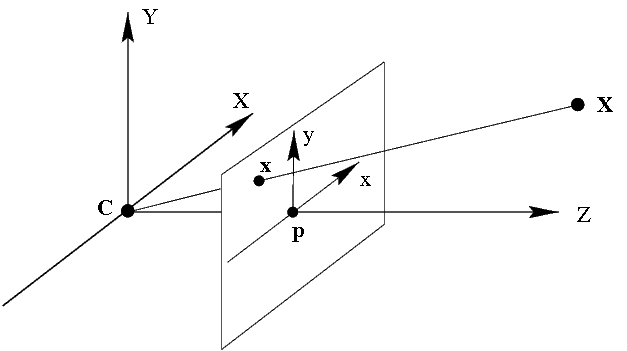
\includegraphics[width=0.7\linewidth]{camera_model.png}
				\caption{Модель камеры.}
				\label{fig:cameramodel}
			\end{figure}

			Формула проецирования для идеальной камеры имеет простую математическую запись в однородных координатах:
			\[x = P X\]
			где \(X\) — однородные координаты точки пространства, \(x\) — однородные координаты точки плоскости, \(P\) — \textit{матрица камеры} размера \(3 \times 4\).
			Однако, в случае более сложных камер, искажения, вносимые линзами, могут сильно повлиять на результат. В результате функция проецирования принимает более сложный вид и часто записывается как последовательность преобразований.

			\paragraph{Дисторсия.} В силу неидеальности оптики, на изображениях, полученных с камер, присутствуют искажения-дисторсии (\textit{\textbf{distortion}}). Данные искажения нелинейны, однако могут быть вычисленны.

			В результате дисторсии в действительности прямые линии становятся кривыми на изображении, кроме линий, лежащих в одной плоскости с главной осью. Дисторсии не зависят от расстояния до объекта, а зависят только от координат точек, в которые проецируются пиксели объекта. Следовательно, для компенсации дисторсий обычно выполняется преобразование исходного изображения полученного с камеры. Это преобразование будет одним и тем же для всех изображений, полученных с камеры, при условии постоянства фокусного расстояния.

			\paragraph{Калибровка.} В ситуации, когда известны внутренние параметры камеры и коэффициенты дисторсии, говорят, что камера откалибрована. Матрица камеры \(P\) неявно содержит в себе все эти параметры.

			Калибровка камер обычно выполняется за счет многократной съемки некоторого калибровочного шаблона, на изображении которого можно легко выделить ключевые точки, для которых известны их относительные положения в пространстве. Далее составляются и решаются (приближенно) системы уравнений, связывающие координаты проекций, матрицы камер и положения точек шаблона в пространстве. Таким образом находятся все необходимые параметры.

			Существует несколько различных подходов к решению задачи калибровки:
			\begin{itemize}
				\item Классический подход — алгоритм Roger Y. Tsai~\cite{Tsai1984}. Он состоит из двух этапов: на первом определяются параметры внешней калибровки; на втором — внутренней калибровки и дисторсии. \textit{Параметры внутренней  калибровки}: фокусное расстояние, угол наклона пикселей и \textit{принципиальная точка} (точка пересечения плоскости изображения с оптической осью, совпадающая с центром фотографии. В реальных камерах, как правило, бывает немного смещена из-за оптических искажений). \textit{Параметры внешней калибровки} задают положение камеры в мировой системе координат. Параметры внешней калибровки связаны непосредственно с фотографируемой сценой, поэтому (в отличие от параметров внутренней калибровки) каждой фотографии соответствует свой набор этих параметров.

				\item Новая гибкая технология калибровки камеры, которая была разработана Zhengyou Zhang~\cite{Zhang2000} и основана на использовании плоского калибровочного объекта в виде шахматной доски.

				\item Автокалибровка — получение калибровочных данных непосредственно по изображениям, причём в сцене не требуется присутствие специальных калибровочных объектов \cite{Frey}.
			\end{itemize}

			Существуют общедоступные реализации алгоритмов калибровки, например, Matlab Calibration toolbox. Библиотека OpenCV также включает в себя алгоритмы калибровки камер и поиска калибровочного шаблона на изображении. Более подробно о калибровке см.~\cite{Hartley2003}.

			\paragraph{Пара камер.} Об определении трехмерных координат наблюдаемых точек можно говорить, когда есть как минимум две камеры.

			Если имеются две камеры, заданные своими матрицами \(P\) и \(P'\) в некоторой системе координат, в таком случае говорят, что имеется пара откалиброванных камер. Если центры камер не совпадают, то эту пару камер можно использовать для определения трехмерных координат наблюдаемых точек.

			\paragraph{Эпиполярная линия.} Перед тем как перейти к описанию метода вычисления трехмерных координат точек, рассмотрим некоторые важные геометрические свойства, связывающие положения проекций точки трехмерного пространства на изображениях с различных камер.

			\begin{figure}[h]
				\centering
				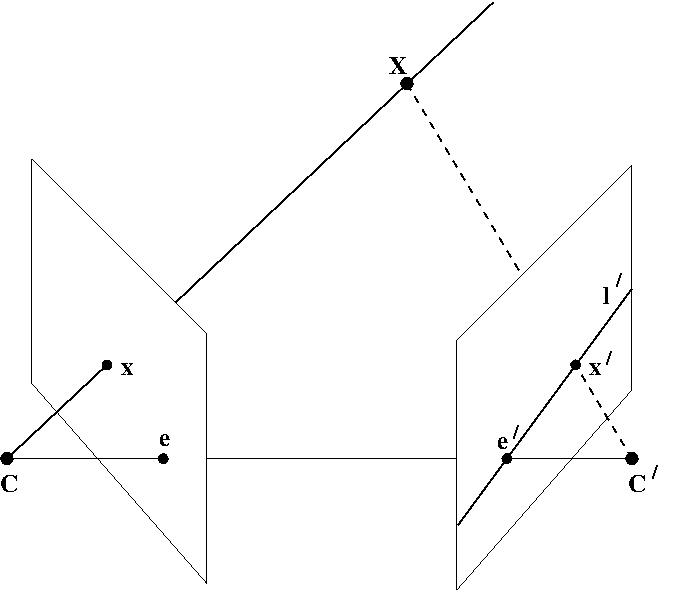
\includegraphics[width=0.5\linewidth]{epipolar_geom.png}
				\caption{Эпиполярная геометрия}
				\label{fig:epipolargeom}
			\end{figure}

			Пусть имеются две камеры, как изображено на Рис.~\ref{fig:epipolargeom}: \(C\) — центр первой камеры, \(C'\) — центр второй камеры. Точка пространства \(X\) проецируется в \(x\) на плоскость изображения левой камеры и в \(x'\) на плоскость изображения правой камеры. Изображения, полученные левой и правой камерами, будем называть \textit{базовым изображением} и \textit{парным изображением} соответственно.

			Прообразом точки \(x\) на изображении левой камеры является луч \(xX\). Этот луч проецируется на плоскость второй камеры в прямую \(l'\), называемую \textit{эпиполярной линией} (\textbf{\textit{epiline}}). Образ точки \(X\) на плоскости изображения второй камеры обязательно лежит на эпиполярной линии~\(l'\).

			Таким образом, каждой точке \(x\) на базовом изображении соответствует эпиполярная линия \(l'\) на парном изображении. При этом пара для \(x\) на парном изображении может лежать только на соответствующей эпиполярной линии. Аналогично, каждой точке \(x'\) на парном изображении соответствует эпиполярная линия \(l\) на базовом.

			Эпиполярную геометрию используют для поиска стереопар, и для проверки того, что пара точек может быть \textit{стереопарой} (т.е. проекцией некоторой точки пространства).

			\paragraph{Фундаментальная матрица.} Пусть имеется пара откалиброванных камер, и пусть \(x\) — однородные координаты точки на изображении одной камеры, а \(x'\) — на изображении второй. Существует такая матрица \(F\) размера \(3 \times 3\), что пара точек \(x\), \(x'\) является стереопарой тогда и только тогда, когда \(x'^{\text{ }T} F x = 0\).

			Матрица \(F\) называется \textit{фундаментальной матрицей} (\textbf{\textit{fundamental matrix}}). Ее ранг равен двум, и она зависит только от матриц исходных камер \(P\) и \(P'\). В главе «Computation of Fundamental Matrix» книги \cite{Hartley2003} можно найти различные алгоритмы вычисления \(F\) по набору точек.

			С помощью фундаментальной матрицы вычисляются уравнения эпиполярных линий. Для точки \(x\), вектор, задающий эпиполярную линию, будет иметь вид \(l' = F x\), а уравнение самой эпиполярной линии: \(l'^{\text{ }T} x' = 0\). Для точки \(x'\), вектор, задающий эпиполярную линию, будет иметь вид \(l = F^{T} x'\).

			\paragraph{Существенная матрица.} Помимо фундаментальной матрицы, существует еще такое понятие, как \textit{существенная матрица}  (\textit{\textbf{essential matrix}}) (часто обозначают \(E\)). По существенной матрице можно восстановить положение и поворот второй камеры относительно первой, поэтому она используется в задачах, в которых нужно определить движение камеры.

			\paragraph{Триангуляция точек.} Процесс определения трехмерной координаты точки по координатам ее проекций называется \textit{триангуляцией} (\textit{\textbf{triangulation}}).

			Для нахождения трехмерной координаты точки необходимо решить следующую систему уравнений:
			\begin{equation}
				\begin{cases}
					x = PX,\\
					x' = P'X.
				\end{cases}
			\end{equation}

			\paragraph{Ректификация.} Как уже говорилось, парную точку \(x'\) для точки \(x\) нужно искать на эпиполярной линии. Соответственно, для упрощения поиска изображения выравнивают так, чтобы все эпиполярные линии были параллельны сторонам изображения (обычно горизонтальны). Более того, изображения выравнивают так, чтобы для точки с координатами \(\left(x_0, y_0\right)\) (в системе координат изображения) соответствующая ей эпиполярная линия задавалась уравнением \(y = y_0\), тогда для каждой точки соответствующую ей парную точку нужно искать в той же строчке на изображении со второй камеры. Такой процесс выравнивания изображений называют \textit{ректификацией} (\textit{\textbf{rectification}}). Ректификация позволяет сузить двумерное пространство поиска решений для проблемы соответствия точек до одного измерения. Другими словами: после проведения ректификации, все пиксели изображения с правой камеры, которые могут соответствовать данной точке изображения с левой камеры, будут находиться в одной сроке.

			\paragraph{Карта диспаратности.} Рассмотрим Рис.~\ref{fig:stereodepth}. Пусть \(X\) -- наблюдаемый объект; \(B\) -- расстояние между камерами (\textit{стереобаза}); \(f\) -- фокусное расстояние камер (будем полагать, что одно и то же для двух камер); \(x_{pr}\), \(x'_{pr}\)  -- евклидовы координаты проекций точек \(x\); \(x'\) на ось \(OO'\); \(z\) -- расстояние от точки \(X\) до прямой \(OO'\). Воспользовавшись подобием треугольников \(OXO' \sim xXx'\) легко получить:
			\begin{equation}
			B-\left(x'_{pr}-x_{pr}\right) = \frac{Bf}{z}.
			\label{eq:1}
			\end{equation}

			\begin{figure}[h]
				\centering
				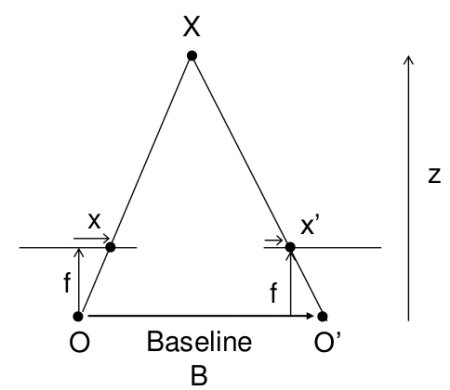
\includegraphics[width=0.4\linewidth]{stereo_depth.jpg}
				\caption{Поясняющий рисунок}
				\label{fig:stereodepth}
			\end{figure}

			Если \(x_{img}\), \(x'_{img}\) -- евклидовы координаты точки \(X\) в системе координат изображений с левой и правой камеры соответственно, то, очевидно, что они следующим образом связаны с координатами проекций на ось \(OO'\):
			\[ x_{img} = x_{pr}, \]
			\[ x'_{img} = -\left(B - x'_{pr}\right). \]

			Подставляя последние выражения в \eqref{eq:1}, получим:
			\begin{equation}
			\left( x_{img}-x'_{img} \right) = \frac{Bf}{z}.
			\label{eq:2}
			\end{equation}

			\textit{Диспарантностью}, \textit{смещением или диспаритетом} (\textbf{\textit{disparity}}) называют величину \(d\), которая задается выражением:
			\begin{equation}
			d = x_{img}-x'_{img}.
			\label{eq:d_x}
			\end{equation}
			Исходя из этого, выражение \eqref{eq:2} можно переписать следующим образом:
			\begin{equation}
			d = \frac{Bf}{z}.
			\label{eq:d_z}
			\end{equation}
			Очевидно, что точки, расположенные дальше от плоскости стереопары, имеют меньшее значение диспаратности, и наоборот. Также с увеличением расстояния \(B\) между камерами, значение диспаратности увеличивается. Из-за обратной зависимости глубины \(z\) и смещения \(d\), разрешающая способность систем стерео зрения, которые работают на основе данного метода, лучше на близких расстояниях, и хуже на далеких.

			Если найти точечные соответствия между изображениями, полученными с разных камер, то с помощью формулы \eqref{eq:d_x} без труда можно найти диспаратность \(d\) для каждой точки на изображении.

			После ректификации изображений, выполняют поиск соответствующих пар точек. Существуют различные способы поиска точечных соответствий \cite{Parchami2014}. Самый простой способ состоит в следующем. Для каждого пикселя левой картинки с координатами \((x_0, y_0)\) выполняется поиск пикселя на правой картинке. При этом предполагается, что пиксель на правой картинке должен иметь координаты \((x_0 - d, y_0)\), где \(d\) -- диспаратность. Поиск соответствующего пикселя выполняется путем вычисления максимума функции отклика, в качестве которой может выступать, например, корреляция окрестностей пикселей. В результате находится диспаратность и строится карта смещений.

			\textit{Картой диспаратности} или \textit{картой смещений} (\textbf{\textit{disparity map}}) называется изображение, полученное в результате вычисления диспаратности для каждой точки на исходных изображениях. Значение яркости в каждой точке такого изображения будет равно вычисленной диспаратности в этой точке.

			На карте диспаратности могут существовать точки, в которых не удалось найти диспаратность, такие точки называются \textit{точками разрыва диспаритета}.
			Области, в которых диспаритет терпит разрыв, обычно заполняют. Например, находят ближайшие к точке разрыва «значащие» пиксели слева и справа вдоль строки и присваивают точке разрыва наименьший из двух диспаритетов, т.е. значение диспаритета в области фона. После заполнения пустот карту диспаритета можно сгладить, например, медианным фильтром

			\paragraph{Карта глубины.} \textit{Карта глубины} (\textit{\textbf{depth map}}) — это изображение, на котором в каждом пикселе, вместо цвета, храниться расстояние до камеры. Карта глубины может быть получена с помощью специальной камеры глубины (например, сенсор Kinect является своего рода такой камерой), а также может быть построена по стереопаре изображений \cite{Bradski2008}.

			По известной карте диспаратности с помощью выражения \eqref{eq:d_z}, можно найти расстояние \(z\) до точек на сцене, фотографии которой рассматриваются. Однако для этого требуется знать расстояние \(B\) между камерами и фокусное расстояние камер \(f\), которое можно найти при помощи калибровки. Причем, поскольку фокусное расстояние и расстояние между камерами остаются постоянными для всех точек на фотографии, то диспаратность можно использовать как относительную глубину точек.

			Один из возможных алгоритмов вычисления расстояния до наблюдаемого объекта можно записать следующим образом \cite{Ilyasov2016}:

			\begin{enumerate}
				\item Производится сбор изображений, на которых изображен шаблон шахматной доски в различных положениях, с левой и правой камер стереопары. Для корректной работы реализации алгоритма необходимо, чтобы шаблон шахматной доски полностью попадал в область видимости камер стереопары и занимал как можно большую площадь кадра. \label{it:1}

				\item Производится поиск узлов шаблона шахматной доски на изображениях полученных на шаге~\ref{it:1}. Поиск узлов шаблона можно осуществить при помощи функции библиотеки OpenCV \texttt{cv::findChessboardCorners()}. Координаты узлов шаблона сохраняются для дальнейшего использования. \label{it:2}

				\item Производится калибровка каждой из стереопар по отдельности. Калибровка камер стереопары осуществляется при помощи функции \texttt{cv::calibrateCamera()}. \label{it:3}

				\item Производится калибровка всей стереопары. Данные, полученные на предыдущем шаге подаются на вход функции \texttt{cv::stereoCalibrate()}, которая считает внутренние параметры стереопары. После процедуры стерео калибровки мы получаем фокусное расстоянии камер, координаты принципиальных точек камер и величину стереобазы. \label{it:4}

				\item Производится ректификация изображений, полученных на шаге \ref{it:1}. Ректификация заключается в выравнивании деформированных изображений, таким образом, чтобы эпиполярные линии изображений с левой камеры совпадали с эпиполярными линиями изображений с правой камеры. Данную процедуру выполняет функция \texttt{cv::stereoRectify()}. \label{it:5}

				\item Производится устранение дисторсии на изображениях шахматной доски, полученных на шаге~\ref{it:5}. Устранение дисторсии производится при помощи функций \texttt{cv::initUndistortRectifyMap()} и \texttt{cv::remap()}. После выполнения данного шага, все прямые линии наблюдаемых объектов на сцене становятся прямыми линиями на изображении. \label{it:6}

				\item Для каждой пары соответствующих изображений с левой и правой камер производится построение карты диспаратностей по изображениям, полученным на шестом шаге. Каждый пиксель карты диспаратностей, в действительности, содержит в себе информацию о том, сколько пикселей по оси \(OX\) находится между соответствующими пикселями изображений объекта с левой и правой камер. Построение карты диспаратностей может быть осуществленно на основе алгоритма SGM \cite{Hirschmuller2008} при помощи класса \texttt{cv::StereoSGBM}. \label{it:7}

				\item Производится вычисление расстояний до наблюдаемых на сцене объектов (см. формулу \eqref{eq:d_z}). Вычисление расстояния до объекта напрямую связано с информацией, которую несет в себе карта диспаратностей, построенная на шаге~\ref{it:7}, и информацией полученной в результате калибровки на шаге~\ref{it:6}. \label{it:8}
			\end{enumerate}

		\subsection{Алгоритмы построения карты диспаратности}
		\label{subsec:disp_algs}
			В данном разделе содержатся базовые сведения об алгоритмах построения карты диспаратности.

			Для построения карты диспаратности необходимо найти точечные соответствия между изображениями с разных камер. Только лишь эпиполярного ограничения (ректификации) и предположения	о соответствии цветов соответствующих точек недостаточно, так как задача остается	некорректно поставленной, потому что:
			\begin{itemize}
				\item Решение может не существовать (перекрытия);
				\item Решение может быть не уникально (однородные области);
				\item Небольшие изменения входных данных существенно влияют на результат (шум).
			\end{itemize}
			По этой причине существуют различные методы, которые используют дополнительные ограничения и предположения.

			Различают два достаточно широких класса алгоритмов для решения проблемы соответствия: \textit{локальные и глобальные алгоритмы}.

			Вычислительная сложность локальных алгоритмов невысока, однако результат работы может содержать ошибки, которые, в свою очередь, могут оказаться неприемлемыми для некоторых приложений. Алгоритмы называются локальными, так как диспаритет в каждой точке зависит только от ее локальной окрестности.

			Глобальные алгоритмы, как правило, показывают хорошие результаты, но из-за высокой вычислительной сложности использовать их в реальном времени практически невозможно. Алгоритмы называются глобальными, так как диспаритет в каждой точке вычисляется при помощи некоторой глобальной процедуры оптимизации, то есть зависит не только от локальной окрестности.

			В сумме эти два класса алгоритмов объединяют большинство из существующих решений. Большинство алгоритмов выполняют, частично или полностью, следующие шаги \cite{Scharstein2002}:
			\begin{enumerate}
				\item Вычисление меры соответствий.
				\item Суммирование мер соответствий.
				\item Вычисление диспаратностей на основе вычисленных мер.
				\item Улучшение карты диспаратности.
			\end{enumerate}
			Реальная последовательность шагов зависит от конкретного алгоритма. Под \textit{мерой соответствий} понимают величину, которая характеризует схожесть между двумя областями на изображениях с разных камер. Мера соответствий используется для того, чтобы уменьшить количество неправильно найденных соответствий. Меру соответствий также называют \textit{стоимостью соответствий}. Существуют различные подходы вычисления меры, многие из которых основанны на значениях интенсивности пикселей. Например, такие способы, как нахождение абсолютной разности интенсивностей (Absolute Intensity Differences, AD) и квадрата разности интенсивностей (Squared Intensity Differences, SD).

			\paragraph{Локальные алгоритмы.} Этот класс алгоритмов подсчитывает диспаратность каждого пикселя в отдельности, используя окна фиксированного или адаптируемого размера для корреляции. Выбор формы окна и его размеров является непростой задачей.

			Для локальных алгоритмов мера соответствия (т.е. первый шаг работы алгоритма) определяется как схожесть между двумя областями, одна из которых находится в базовом изображении, а	другая -- в парном. Форма этих областей зависит от конкретного алгоритма. Стандартные	подходы, появившиеся на заре исследований проблемы соответствия, используют прямоугольное окно фиксированного размера. Размеры этого окна определяются опытным путем. Объем вычислений, в этом случае, сильно сокращается по сравнению с современными	методами, но существует ряд проблем, избежать которых, используя	фиксированный размер окна, практически невозможно. Маленькие окна приводят к недостаточной информации о текстуре области, в связи с чем возникает большая чувствительность к шумам. При использовании большого окна возникает эффект «раздувания» объектов	переднего плана (\textit{foreground fattening}) при однотонных фонах. Существуют алгоритмы, решающие эту проблему с помощью адаптивного размера окна. Развитие локальных методов на сегодняшний день идет в различных направлениях. Среди которых можно выделить: направление адаптивных окон; алгоритмы, которые используют сегментацию изображения и исходят из предположения, что области разрыва диспаритета совпадают с краями (границами сегментов) на изображении; алгоритмы, которые используют вероятностные модели, например алгоритм ELAS \cite{Geiger2010}.


			После того, как для каждого пикселя подсчитана мера соответствия, локальный алгоритм, обычно, переходит к шагу суммирования мер. Стандартный подход состоит в суммировании или усреднении мер соответствия в некоторой области. Усреднение может производиться с помощью свертки с каким-нибудь ядром, чаще всего Гауссовым.

			Финальным шагом является вычисление диспаратности на основе просуммированных или усредненных мер соответствий. Диспаратность для данного пикселя базового изображения – это значение, на котором достигается минимальное значение меры (или максимальное, в зависимости от выбранной меры). Проблема, возникающая при таком подходе,	состоит в том, что каждой точке выбирается уникальное соответствие на парном изображении, но на самом же деле, одной точке может соответствовать сразу несколько. К сожалению, эта	проблема возникает не только у локальных алгоритмов, но и у подавляющего большинства	методов, целью которых является построение карты диспаратности.

			\paragraph{Глобальные алгоритмы.} В отличие от локальных алгоритмов, где нахождение диспаратности происходит для каждого	пикселя отдельно, целью глобального подхода является поиск наилучшей карты	диспаратности для всего изображения сразу. Глобальные алгоритмы практически всю работу	выполняют на шаге вычисления диспаратностей, часто пропуская шаг суммирования мер соответствия. Чаще всего глобальные алгоритмы решают проблему соответствия путем минимизации некоторого функционала энергии.
			Глобальные алгоритмы -- наилучшие по качеству методы на сегодняшний день. Количество ошибок, допускаемых ими, относительно невелико. Тем не менее, большинство глобальных алгоритмов непригодны для работы в реальном времени \cite{Scharstein2002}.

			\begin{figure}[h]
				\minipage{0.32\textwidth}
				\centering
				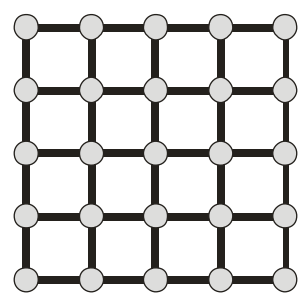
\includegraphics[width=0.8\linewidth]{graph_0.png}
				\caption{Схема графа решетки.}
				\label{fig:graph_0}
				\endminipage\hfill
				\minipage{0.32\textwidth}
				\centering
				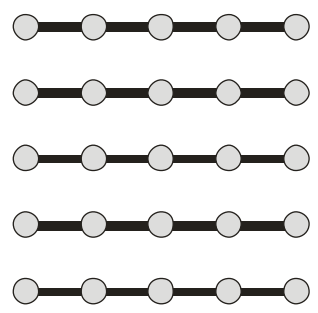
\includegraphics[width=0.8\linewidth]{graph_1.png}
				\caption{Схема графа в \cite{Jung2006}.}
				\label{fig:graph_1}
				\endminipage\hfill
				\minipage{0.32\textwidth}
				\centering
				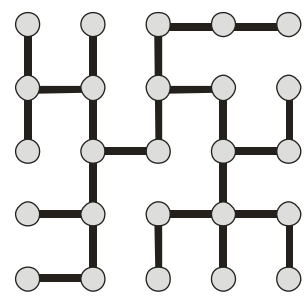
\includegraphics[width=0.8\linewidth]{graph_2.png}
				\caption{Схема графа в \cite{Veksler2005}.}
				\label{fig:graph_2}
				\endminipage\hfill
			\end{figure}
			\begin{figure}[h]
				\minipage{0.32\textwidth}
				\centering
				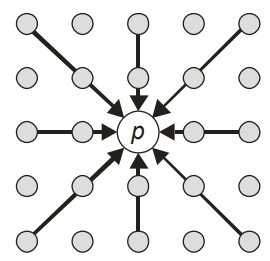
\includegraphics[width=0.8\linewidth]{graph_3.png}
				\caption{Схема графа в SGM \cite{Hirschmuller2008}.}
				\label{fig:graph_3}
				\endminipage\hfill
				\minipage{0.7\textwidth}
				\centering
				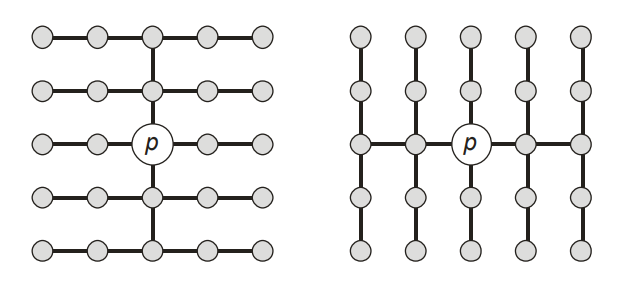
\includegraphics[width=0.8\linewidth]{graph_4.png}
				\caption{Схема графа в  \cite{Bleyer2008}.}
				\label{fig:graph_4}
				\endminipage\hfill
			\end{figure}
			Как правило, глобальные алгоритмы формулируются в терминах разметки графа и минимизации энергии. Рассматривается граф (решетка, см.~Рис.~\ref{fig:graph_0}) , где метки – значения диспаритета, узлы – пиксели. Осуществляется поиск разметки \(D\), минимизирующей функцию энергии	\(E(D)\):
			\begin{equation}
			E\left(D\right) = E_{data}\left(D\right)+E_{smooth}\left(D\right),
			\end{equation}
			где \(E_{data}\left(D\right)\) – унарный потенциал, который характеризует степень согласованности конфигурации с парой входных изображений и вычисляется с помощью мер соответствия; \(E_{smooth}\left(D\right)\) – парный потенциал, который явным образом реализует предположение о гладкости, т.е. накапливает величину штрафа, налагаемого на данную конфигурацию при нарушении гладкости диспаратностей. Обычно при вычислении парного потенциала учитываются соседние пиксели. В результате минимизации функционала находится карта диспаратности \(D\).

			Развитие глобальных алгоритмов заключается в уходе от графов	общего вида и переходу к деревьям. Отсутствие циклов в деревьях позволяет использовать метод	динамического программирования и повысить скорость работы алгоритма.

			Существует также разделение глобальных алгоритмов по способу минимизации
			энергии. Чаще всего используется либо динамическое программирование, либо нахождение минимального разреза графов (graph cuts). Алгоритмы разреза графов также получили название двумерных. Их производительность ниже, но результаты имеют более высокую точность. В ходе использования одномерных алгоритмов строки изображений обрабатываются независимо друг от друга. Вследствие этого их	скорость выше, но возникает эффект «гребенки» – рассогласование значений диспаратности на уровне отдельных строк.

			Так, например, в алгоритме Scanline Optimization \cite{Jung2006} удаляются все вертикальные ребра (Рис.~\ref{fig:graph_1}). Алгоритм работает, однако рассогласованность строк между собой (\textit{horizontal streaking}) вносит в результат заметные искажения. Алгоритм, предложенный в работе \cite{Veksler2005}, учитывает связь различных строк и основан на построении минимального покрывающего дерева (Рис.~\ref{fig:graph_2}). Результат улучшается, однако некоторая рассогласованность всё-таки остается.

			Другой популярный алгоритм -- SGM, описан в работе \cite{Hirschmuller2008}. Подход не совсем глобальный, но и не локальный. Алгоритм SGM дает практически такие же результаты, как и глобальные алгоритмы, однако скорость его работы гораздо выше. В каждом пикселе строится свое дерево (Рис.~\ref{fig:graph_3}). Оптимизация производится вдоль лучей, исходящих из пикселя. Рассогласованности нет, но могут присутствовать «изолированные» пиксели, резко отличающиеся от соседних с ними пикселей. Такие пиксели могут быть удалены различными способами на этапе постобработки.

			Алгоритм Simple Tree, предложенный в \cite{Bleyer2008}, лишен недостатка SGM. В нем предлагается в каждом пикселе строить два дерева (Рис.~\ref{fig:graph_4}), совместно покрывающих все
			изображение.

			Сравнительный анализ эффективности алгоритмов показывает, что метод SGM показывает наилучшие результаты с точки зрения быстродействия, качественной и количественной оценки полученных карт диспаратности \cite{Ponomarev2013}.

			\paragraph{StereoBM.} В библиотеке OpenCV \cite{Bradski2000}	реализованны алгоритмы StereoSGBM и StereoBM.

			Алгоритм StereoBM производит некоторую предобработку изображений. Построчно анализирует базовое и парное изображение. На каждой строке алгоритм берет точку или их набор, и пытается найти похожий набор точек на этой же строчке на правом изображении. После этого он считает, насколько эти наборы точек друг относительно друга смещены. На последнем шаге проводится некоторая пост обработка и в результате получается карта диспаритета.

			На вход функции \texttt{cv::StereoBM} подаются базовое и парное изображения и два параметра -  \texttt{ndisparities} и \texttt{SADWindowSize}. Первый параметр \texttt{ndisparities} указывает, насколько "далеко"\ алгоритм должен просмотреть строчку парного изображения в поисках нужного ему фрагмента. Если указать \texttt{ndisparities = 16}, то это будет означать, что алгоритм будет "заглядывать"\ левее на 16 пикселей.
			Параметр \texttt{SADWindowSize} -- это размер окна, который алгоритм будет использовать для вычисления меры соответствия.

			StereoBM -- алгоритм, работающий в реальном времени (может обрабатывать изображение \(1920 \times 1080\) в миллисекундах). StereoBM работает  быстрее, но является менее точным по сравнению с StereoSGBM. Как показывают эксперименты, некоторая предобработка исходных изображений улучшает качество работы алгоритма и приближает его к качеству алгоритма StereoSGBM (см.~\cite{Parchami2014}).

			\paragraph{StereoSGBM.} StereoSGBM является более точным алгоритмом, но работает медленней (несколько секунд, для изображения \(1920 \times 1080\)).

			Реализация алгоритма StereoSGBM в библиотеке OpenCV несколько отличается от оригинального алгоритма SGM, описанного в \cite{Hirschmuller2008}, а именно:
			\begin{itemize}
				 	\item По умолчанию алгоритм рассматривает 5 направлений суммирования стоимостей соответствий вместо 8. Для рассмотрения 8 направлений необходимо установить параметр \texttt{mode=StereoSGBM::MODE\_HH}.

				 	\item Алгоритм сравнивает блоки, а не пиксели. Для сравнения пикселей необходимо установить параметр \texttt{blockSize=1}.

				 	\item Вместо предлагаемой в работе меры соответствия использована более простая мера Birchfield-Tomasi \cite{Birchfield1998}, которая устойчива к погрешности сэмплирования (когда непрерывный сигнал может быть сэмплирован по-разному, из-за чего цвета соответствующих пикселей на разных изображениях могут не совпасть).

				 	\item Используется некоторая пре- и пост- обработка, как и в реализации алгоритма StereoBM.
			\end{itemize}

		 	Параметры алгоритма StereoSGBM:
		 	\begin{itemize}
		 		\item \texttt{minDisparity}	-- минимально возможное значение диспаритета. Обычно значение равно нулю, однако иногда процедура ректификации может смещать изображения, поэтому этот параметр можно соответствующим образом отрегулировать.

			 	\item \texttt{numDisparities} -- модуль разности максимального и минимального значения диспаритета. В текущей реализации значение данного параметра должно делиться на 16.

			 	\item \texttt{blockSize} -- размер сравниваемых блоков. Нечетное число больше 1. Обычно размер выбирается в промежутке \(3 \dots 11\).

			 	\item \texttt{P1} -- первый параметр, контролирующий сглаживание диспаритета.

			 	\item \texttt{P2} -- второй параметр, контролирующий сглаживание диспаритета. Чем больше значение, тем больше сглаживание. \texttt{P1} -- это величина штрафа в случае, если диспаритет изменяется на \(\pm 1\) между соседними пикселями в окне заданного размера. \texttt{P2} -- это величина штрафа в случае, если диспаритет изменяется более чем на \(1\) между соседними пикселями в окне заданного размера.
			 	Алгоритм требует выполнения условия \texttt{P2 > P1} . Относительно хороший результат дают следующие значения:

			 	\begin{center}
			 		\texttt{P1} \(=8 \cdot \texttt{number\_of\_image\_channels} \cdot \texttt{SADWindowSize}^{2},\)

			 		\texttt{P2} \(=32  \cdot \texttt{number\_of\_image\_channels} \cdot \texttt{SADWindowSize}^{2}.\)
			 	\end{center}

			 	\item \texttt{disp12MaxDiff} -- максимально допустимая разность (в единицах целочисленного пикселя) в диспаритете для левого-правого изображений. Отрицательное значение отключает такую проверку.

			 	\item \texttt{preFilterCap} -- значение порога усечения для предварительно фильтрованных пикселей изображения. Алгоритм сначала вычисляет производную по \(x\) на каждом пикселе и фиксирует это значение на интервале [-\texttt{preFilterCap}, \texttt{preFilterCap}]. Значения результата передаются в функцию расчета меры соответствий Birchfield-Tomasi.

			 	\item \texttt{uniquenessRatio} -- запас в процентах, по который лучшее (минимальное) значение меры соответствий должно «выиграть» у второго лучшего значения, чтобы считать найденное совпадение правильным. Обычно значение в пределах диапазона 5-15 достаточно хорошее.

			 	\item \texttt{speckleWindowSize} -- Максимальный размер областей гладких регионов диспаритета для поиска и удаления шумовых пятен. Значение 0 отключает фильтрацию пятен. Обычно рабастные значение лежат в пределах диапазона 50-200.

			 	\item \texttt{speckleRange}	-- максимальное различие в каждой области. При выполнении фильтрации пятен параметр имеет положительное значение, которое будет неявно умножено на 16. Обычно устанавливают значения 1 или 2.

			 	\item \texttt{mode}	-- режим работы. Возможные значения: \texttt{StereoSGBM::MODE\_SGBM}, \texttt{StereoSGBM::MODE\_HH }, \texttt{StereoSGBM::MODE\_SGBM\_3WAY }, \texttt{StereoSGBM::MODE\_HH4}. Значение \texttt{StereoSGBM::MODE\_HH}, запускает полномасштабный двухпроходный алгоритм динамического программирования. Алгоритм будет потреблять \(O \left(W \cdot H \cdot \texttt{numDisparities}\right)\), которые являются большими для изображений 640x480 и огромны для HD-изображений. По умолчанию установлено значение \textit{False}.
		 	\end{itemize}

	 	\subsection{Алгоритм нахождения свободных для движения регионов}
	 	\label{subsec:tr_reg_alg}
	 		В этом разделе рассмотрим алгоритм, предложенный в работе \cite{Zhu2013} и использующий u-v-диспаритет.

	 		Детекция регионов, доступных для движения, является важной задачей для навигации мобильных роботов и беспилотных транспортных средств. Препятствия, которые делают регион недоступным для движения, можно разделить на два основных класса: 1) геометрические препятствия; 2) не геометрические препятствия (связанны, например,  со свойством поверхности: вязкость, малая плотность, неровность).
	 		Данная задача может решаться на основе данных полученных с разных источников:  лазерного сканера (LIDAR) , стерео камер, 2D датчиков глубины и других.

	 		Можно выделить два основных подхода к детекции регионов, доступных для движения, на основе данных, полученных со стерео камер:
		 	\begin{enumerate}
		 		\item Проведение 3D реконструкции по облаку точек, полученному на основе карты диспаритета, и с последующее использование детекции углов, поиска плоскостей и других характеристик для нахождения регионов, доступных для движения, и регионов с препятствиями~\cite{Li2007, Murarka2008, Braun2008}. Преимуществом такого подхода является хорошая точность. Недостатком -- высокая сложность вычислений и, как следствие, невозможность работы в приложениях реального времени.

		 		\item Использование u-v-диспаритета \cite{Labayrade2002, Broggi2005, Hu2005}. Преимуществом такого подхода является скорость вычислений.
		 	\end{enumerate}

	 		\paragraph{v-диспаритет.}  Пусть \(v\) представляет собой в координату пикселя в \(\left(u,v\right)\) системе координат изображения карты диспаритета, \(d\) -- значение диспаритета. Карта \(v\)-диспаритета строится таким образом, что каждый её пиксель с координатами \(\left(d,v\right)\) имеет значение интенсивности равное количеству пикселей с параметрами \(d,v\) на карте диспаритета. Другими словами, \(v\)-диспаритет получается на основе карты диспаритета, подсчетом  количества пикселей в строке \(v\), имеющих одно и то же значение диспаритета \(d\).

	 		Так, например, тот факт, что для вертикального препятствия, удаленного на некоторое расстояние, диспаритет остается постоянным, на карте \(v\)-диспаритета будет отражен в виде вертикальной линии, значение интенсивности которой будет характеризовать ширину препятствия.
	 		Ровная поверхность, такая как дорога, на карте \(v\)-диспаритета также будет отражена ввиде линии, только уже не вертикальной, а наклоненной. Такая линия называется \textit{линией корреляции земли} и она соответствует региону, доступному для движения.

	 		Таким образом, чтобы найти регион, доступный для движения, нужно найти линию корреляции земли и пиксели на карте диспаритета, которые ей соответствуют. Это не сложно сделать с помощью преобразования Хафа, однако присутствие на карте \(v\)-диспаритета линий соответствующих препятствиям значительно ухудшает результат. В работе \cite{Zhu2013} предлагают использовать \(u\)-диспаритет для предварительного поиска препятствий, чтобы они не учитывались при построении \(v\)-диспаритета и, как следствие, не мешали определению линии корреляции земли.

	 		\paragraph{u-диспаритет.} Аналогично \(v\)-диспаритету можно определить \(u\)-диспаритет. Карта \(u\)-диспаритета строится таким образом, что каждый её пиксель с координатами \(\left(u,d\right)\) имеет значение интенсивности равное количеству пикселей с параметрами \(u,d\) на карте диспаритета. Другими словами, \(u\)-диспаритет получается на основе карты диспаритета, подсчетом  количества пикселей в столбце \(u\), имеющих одно и то же значение диспаритета \(d\).

	 		Препятствиям на карте \(u\)-диспаритета будут соответствовать горизонтальные линии, интенсивность которых будет характеризовать высоту препятствий. Ровные поверхности, такие как дорога, в данном случае будут иметь малую интенсивность на карте \(u\)-диспаритета.

	 		С использованием \(u\)-диспаритета могут быть найдены линии соответствующие препятствиям. Пиксели на карте диспаритета, соответствующие этим линиям, будут пикселями препятствий и могут не рассматриваться при построении карты \(v\)-диспаритета.


	 		\paragraph{Алгоритм.} Изложим кратко предложенный в работе \cite{Zhu2013} алгоритм:

	 		\begin{enumerate}
	 			\item Построить карту \(u\)-диспаритета для исходной карты диспаратности.

	 			\item Построить бинарное изображение \(u\)-диспаритета. Для каждого пикселя \(\left(u, d\right)\) при условии, что значение интенсивности \(u\)-диспаритета больше некоторого порогового значения, найти пиксели в \(u\) столбце на исходной карте диспаратности, для которых диспаритет равен \(d\). Найденные пиксели пометить как пиксели препятствия (присвоить значение интенсивности 1), остальные -- как потенциальные пиксели региона свободного для движения (присвоить значение интенсивности 0).

	 			\item Применить морфологическую операцию замыкания для связывания областей с небольшими разрывами. После чего удалить небольшие изолированные участки, т.к. они не пригодны для движения.

	 			\item На исходной карте диспаратности найти пиксели, которые соответствуют пикселям препятствия (значение интенсивности 1). Найденные пиксели образуют новую карту диспаратности -- \textit{карту препятствий}. Остальные пиксели образуют \textit{карту не-препятствий}.

	 			\item Построить карту \(v\)-диспаритета для карты диспаратности не-препятствий.

	 			\item Бинаризовать изображение \(v\)-диспаритета с помощью некоторого порога. С помощью преобразования Хафа на  бинаризованном изображении найти линию корреляции земли. Для всех пикселей, лежащих на найденной линии, найти соответствия на карте не-препятствий. Найденные соответствия пометить как область, доступную для движения (присвоить значение интенсивности 1), всем остальным присвоить значение интенсивности 0. Таким образом получается \textit{карта регионов доступных для движения}.

	 			\item  На найденной карте регионов, доступных для движения, удалить небольшие изолированные участки, т.к. они не пригодны для движения.
 			\end{enumerate}


	 	\subsection{KITTI Benchmark Suite}
	 	\label{subsec:benchmark}
	 		В этом разделе рассмотрим бенчмарк для оценки производительности методов нахождения дорожного полотна.

	 		The KITTI Vision Benchmark Suite -- данные и бенчмарк для разработки и оценки производительности методов и алгоритмов для автономных транспортных средств. Даные получены с автомобиля оснащенного стерео камерами, мобильным лазерным сканером и GPS. Также предлагаются бенчмарки для сравнения производительности различных алгоритмов на предоставляемых данных. Среди них есть бенчмарк Road/Lane Detection Evaluation 2013 для оценки производительности алгоритмов определения дороги и полосы движения \cite{Fritsch2013}.

	 		\paragraph{KITTI-ROAD Dataset.}
 			Содержит два набора изображений с левой и правой камер: один тренировочный, с эталонными результатами и калибровочными данными камер; другой тестовый, в котором эталонные результаты отсутствуют. Тестовый и тренировочный наборы содержат изображения трёх классов дорог (см.~Табл.~\ref{tb:kitti_data}). Кроме того,  предоставляются данные мобильного лазерного сканера и GPS, которые могут быть использованы для получения результатов.

	 		\begin{table}
	 			\centering
		 		\caption{Структура KITTI-ROAD Dataset.}
		 		\label{tb:kitti_data}
		 		\begin{tabular}{|c|c|c|c|}
		 			\hline
		 			\textbf{аббревиатура} &  \textbf{тренировочные} & \textbf{тестовые} & \textbf{описание} \\
		 			\hline
		 			UU & 98 & 100 & городские дороги без дорож.разметки \\

		 			UM & 95 & 96 & городские двухполосные с д.разметкой \\

		 			UMM & 96 & 94 & городские многополосные с д.разметкой \\
		 			\hline
		 			URBAN & 289 & 290 & все три вместе \\
		 			\hline
		 		\end{tabular}
 			\end{table}

	 		\paragraph{KITTI-ROAD Benchmark.}
	 		Производительность алгоритмов предлагается оценивать с помощью "вида сверху"\ (BEV). В работе \cite{Fritsch2013} показано, что использование "вида сверху"\ даёт более корректные результаты, чем использование "перспективного вида". Результаты (в нашем случае карта регионов доступных для движения) преобразовываются к "виду сверху" с помощью обратного перспективного преобразования изображения.
	 		Далее в пространстве BEV вычисляются характеристики, дающие оценку работы алгоритма (более подробно см.~\cite{Fritsch2013}):
	 		\[ Precision = \frac{TP}{TP+FP}, \]
	 		\[ Recall = \frac{TP}{TP+FN}, \]
	 		\[ F\text{-measure} = \left( 1+\beta^{2} \right)\frac{Precision \cdot Recall}{\beta^{2} Precision + Recall}, \]
	 		\[ Accuracy = \frac{TP+TN}{TP+FP+TN+FN}, \]
	 		\[ F_{max} = \max_{\tau} F\text{-measure}, \]
	 		\[ Average Precision = \frac{1}{11} \sum_{r \in 0, 0.1, \dots, 1} \max_{\widetilde{r}:\widetilde{r}>r} Precision(\widetilde{r}), \]
	 		где \(\tau\) -- порог бинаризации в случае если результатом (картой доступных для движения регионов) является не бинарное изображение, а изображение, интенсивность пикселей которого равна вероятности; \(TP\), \(FP\), \(TN\), \(FN\) -- количество истинно-положительных, ложно-положительных, истинно-отрицательны, ложно-отрицательных классификаций; \(\beta\) -- коэффициент, который полагается равным 1; \(r\) -- значение \(Recall\), а \(Precision(r)\) -- соответствующее этому значению \(Precision\).

	 		Если результат классификации положительный, и истинное (эталонное) значение тоже положительное, то речь идет об истинно-положительном значении (true-positive).

	 		Если результат классификации положительный, но истинное значение отрицательное, то речь идет о ложно-положительном значении (false-positive).

	 		Если результат классификации отрицательный, и истинное значение тоже отрицательное, то речь идет об истинно-отрицательном значении (true-negative).

	 		Если результат классификации отрицательный, но истинное значение положительно, то речь идет о ложно-отрицательном значении (false-negative).

	 		\(F_{max}\) и \(AP\) (Average Precision) достаточно хорошо характеризуют точность алгоритма по нахождению дороги. Чем ближе они к единице (100\%), тем точнее работает алгоритм.
	 		Бенчмарк предоставляет \textit{development kit}, в котором реализован данный метод оценки производительности.

	\section{Выполнение задания}
		В этой части приведены описание и результаты экспериментов. Исходный код программ размещен на GitHib\footnote{\href{https://github.com/abramenko/traversable-region-detection}{https://github.com/abramenko/traversable-region-detection}}. Данные для экспериментов: KITTI-ROAD Dataset\footnote{\href{http://www.cvlibs.net/datasets/kitti/eval\_road.php}{http://www.cvlibs.net/datasets/kitti/eval\_road.php}}.

		\subsection{Формат данных}

			\paragraph{Базовые и парные изображения:} цветные изображения в формате PNG, 8 бит (\texttt{uint8}), 3 канала (RGB). Имена файлов \texttt{<cat>\_xxxxxx.png}, где \texttt{<cat>}: \texttt{uu}, \texttt{um} или \texttt{umm}.

			\paragraph{Карты диспаратности:} изображения в формате PNG, 16 бит (\texttt{uint16}), 1 канал. Значение 65535 является маркером для невалидных значений диспаритетов. Значения диспаритетов представлены в формате с фиксированной точкой, 4 бита отведено на дробную часть. Таким образом, чтобы получить значение диспаритета, необходимо после чтения изображения поделить результат на 16. Имена файлов соответствуют именам базовых изображений.

			\paragraph{Карты доступных для движения регионов:} изображения в формате PNG, 16 бит (\texttt{uint8}), 1 канал. Значение 255 является маркером регионов доступных для движения.
			Имена файлов \texttt{<cat>\_<type>\_xxxxxx.png}, где \texttt{<type>}: \texttt{road}.

			\paragraph{Карты эталонных результатов:} цветные изображения в формате PNG, 8 бит (\texttt{uint8}), 3 канала (RGB). Канал B содержит карту эталонных результатов (ground truth), канал R содержит допустимые области оценки (valid evaluation
			areas). Имена файлов соответствуют именам карт регионов доступных для движения.

		\subsection{Нахождение карт диспаратности}
			Карты диспаритета находятся для каждой пары базового и парного изображений помощью алгоритма \texttt{cv::StereoSGBM}. После качественной оценки результата, были выбраны следующие параметры алгоритма (подробнее о значениях параметров см.~п.~\ref{subsec:disp_algs}):
			\begin{itemize}
				\item \(\texttt{minDisparity} = 0\);

				\item \(\texttt{numDisparities} = 7 \cdot 16\);

				\item \(\texttt{blockSize} = 5\);


				\item \(\texttt{P1} =8 \cdot \texttt{number\_of\_image\_channels} \cdot \texttt{SADWindowSize}^{2}\);

				\(\texttt{P2} =32  \cdot \texttt{number\_of\_image\_channels} \cdot \texttt{SADWindowSize}^{2}\),

				где \(\texttt{SADWindowSize} = 7\),		\(\texttt{number\_of\_image\_channels} = 3\);

				\item \(\texttt{disp12MaxDiff} = -1\);

				\item \(\texttt{preFilterCap}  = 1\);

				\item \(\texttt{uniquenessRatio}  = 5\);

				\item \(\texttt{speckleWindowSize} = 200\);

				\item \(\texttt{speckleRange} = 1\);

				\item \(\texttt{mode = StereoSGBM::MODE\_SGBM\_3WAY}\).
			\end{itemize}

			Процесс вычисления карт диспаритета реализован в виде скипта \texttt{img2disp.py} (см.~Приложение, стр.~\pageref{app:imgs2disp}). В результате работы алгоритма \texttt{cv::StereoSGBM} получается изображение типа \texttt{int16}. Полученное изображение преобразовывается в тип \texttt{uint16}, а все пиксели, значение диспаритета которых было меньше нуля, помечаются как невалидные (присваивается значение интенсивности равное 65535). Результат вычисленния карты диспаритета для базового и парного изображения (см.~Рис.~\ref{fig:base_img},~\ref{fig:pair_img}) показан на Рис.~\ref{fig:disp_img} на стр.~\pageref{fig:disp_img}. Результаты достаточно хорошие, но их можно улучшить, если провести ректификацию базового и парного изображений.% Я предполагаю, что они не ректифицированны

		\subsection{Нахождение регионов доступных для движения}
			Процесс нахождения доступных для движения регионов реализован в виде скипта \texttt{find\_traversable.py} (см.~Приложение, стр.~\pageref{app:find_traversable}). Реализован алгоритм, описаный в п.~\ref{subsec:tr_reg_alg}. В реализации алгоритма используются следующие параметры:
			\begin{itemize}
				\item \(\texttt{u\_disp\_threshold = 3}\) -- порог для бинаризации \(u\)-диспаритета;

				\item \(\texttt{v\_disp\_threshold = 3}\) --  порог для бинаризации \(v\)-диспаритета;

				\item \(\texttt{morph\_disk\_radius = 9}\) -- размер радиуса диска (в пикселях), который используется как структурообразующий элемент при морфологической операции замыкания.

				\item \(\texttt{small\_obj\_size = 500}\) -- максимальный размер небольших изолированных объектов (в пикселях). Объекты, размер которых меньше зданного, будут удалены.

				\item \(\texttt{line\_width=20}\) -- ширина найденной линии корреляции земной поверхности.
			\end{itemize}

			В скрипте \texttt{find\_traversable.py} нахождение линии корреляции земной поверхности реализовано следующим образом:
			\begin{enumerate}
				\item С помощью преобразования Хафа находятся параметры \(r\), \(\theta\) прямой, набравшей наибольшее количество голосов.

				\item Считается, что пиксель лежит на линии корреляции земной поверхности, если его координаты удовлетворяют неравенству:
				\[r-\frac{\texttt{line\_width}}{2} \leq \left(d \cdot \cos{\theta} + v \cdot \sin{\theta}\right) \leq r + \frac{\texttt{line\_width}}{2} \]
			\end{enumerate}
			Необходимость такой реализации вызвана тем, что за счет различных факторов (ориентация стереокамер, погрешности возникающих при вычислении диспаритета, неровности земной поверхности), линия корреляции земли не является идеальной линией, а имеет форму клина  (см.~Рис.~\ref{fig:gr_corelation} на стр.~\pageref{fig:gr_corelation}). При использовании описанной выше реализации, считается, что пиксель лежит на линии корреляции земли, если он находится между двумя синими сплошными линиями (см.~Рис.~\ref{fig:gr_corelation}), которые удалены на расстояние \(\frac{\texttt{line\_width}}{2}\) от красной пунктирной линии, найденной с помощью преобразования Хафа.

			На Рис.~\ref{fig:u_disp} представлена бинаризованная карта \(u\)-диспаритета, рассчитанная для карты диспаритета базового изображения (см.~Рис.~\ref{fig:disp_img}).
			На Рис.~\ref{fig:obst_disp}, \ref{fig:non_obst_disp} представленны найденные с использованием \(u\)-диспаритета карты препятствий и не-препятствий, соответственно.
			На Рис.~\ref{fig:gr_corelation} представлена бинаризованная карта \(v\)-диспаритета и изображены границы линии кореляции земли.
			Регион доступный для движения, найденный с помощью линии корреляции земли, изображен на Рис.~\ref{fig:img_with_tr_reg} (стр.~\pageref{fig:img_with_tr_reg}).

			Можно заметить, что на Рис.~\ref{fig:img_with_tr_reg} не все плоские регионы (сравните с Рис.~\ref{fig:img_with_tr_reg_100} на стр.~\pageref{fig:img_with_tr_reg_100}) отмечены как регионы доступные для движения.
			Это связано с тем, что линия корреляции земли ищется в виде прямой заданной ширины, в то время как на самом деле она является клином. Эту проблему можно решить, если искать линию корреляции земли в виде клина. Также можно увеличить ширину линии корреляции, например положить \(\texttt{line\_width=100}\), тогда большинство точек клина будут попадать в область между сплошными линиями и регион, доступный для движения, увеличится (см.~Рис.~\ref{fig:img_with_tr_reg_100}).

		\subsection{Оценка результатов работы алгоритма }
			Оценим качество результатов работы алгоритма поиска свободных для движения регионов с помощью методики описанной в п.\ref{subsec:benchmark}. В качестве входных данных используется тренировочный набор данных KITTI-ROAD Dataset. Оценка результатов проводится в BEV пространстве.

			В Таб.~\ref{tb:algs} на стр.~\pageref{tb:algs} приведены результаты вычисления характеристик для карт диспаратности, полученных методами: StereoSGBM~\cite{Hirschmuller2008}, ESGM~ \cite{Hirschmuller2005}, ELAS~\cite{Geiger2010}. Можно видеть, что результаты отличаются незначительно, поэтому можно сделать вывод, что карты диспаритета, рассчитанные разными методами для одних и тех же данных, также отличаются незначительно. Для приложений реального времени целесообразно выбрать быстрый локальный метод ELAS, а в приложениях, где время не критично, можно использовать полу-глобальные методы StereoSGBM или ESGM.

			В Таб.~\ref{tb:l_width} на стр.~\pageref{tb:l_width} приводятся результаты работы алгоритма детекции доступных для движения регионов. Вычисления производились с использованием различных значений параметра \texttt{line\_width}.
			Можно видеть, что из рассмотренных значений параметра наилучшая точность достигается при \(\texttt{line\_width}=5\).
			А наибольшее значение \(F_{max}\) получается для значений \(\texttt{line\_width}\) лежащих на отрезке \(\left[5,20\right]\)

			Полученные характеристики отражают точность и качество нахождения алгоритмом дорожного полотна. В целом алгоритм показывает неплохие результаты, если учитывать то, что он предназначен для обнаружения достаточно плоских участков, по которым теоритически можно проехать, а не только для обнаружения дорожного полотна.

		\subsection{Выводы}
			В ходе работы рассмотрены основные понятия стереозрения, описаны основные подходы к построению карты диспаритета. Реализовано нахождение карты диспаритета с помощью библиотеки OpenCV и алгоритма StereoSGBM. Кратко изложен алгоритм нахождения регионов, доступных для движения. Приведены результаты вычислений и оценка работы алгоритма на данных KITTI-ROAD Dataset.

			Использование стерео камер позволяет в реальном времени решать проблемы навигации беспилотных транспортных средств и мобильных роботов. Однако стереозрение чуствительно к погодным и другим условиям, что приводит к необходимости использовать и данные с других сенсоров. К таким сенсорам можно отнести 3D и 2D лазерные сканеры. Обработка данных, полученных с таких сенсоров занимает больше времени, что не всегда приемлемо с точки зрения безопасности движения. Однако совместное использование данных может помочь качественно улучшить результаты.

	\addcontentsline{toc}{section}{Список литературы}
	\begin{thebibliography}{00}
		\bibitem{Zhu2013} Zhu X. et al. \emph{Stereo vision based traversable region detection for mobile robots using uv-disparity}// Control Conference (CCC), 2013 32nd Chinese. - IEEE, 2013. - pp.~5785-5790.
			\bibitem{Fritsch2013} 	Fritsch J., Kuehnl T., Geiger A. \emph{A New Performance Measure and Evaluation Benchmark for Road Detection Algorithms}// International Conference on Intelligent Transportation Systems (ITSC) -- 2013.
		\bibitem{Bradski2000} Bradski, Gary. \emph{The OpenCV Library}// Dr. Dobb's Journal: Software Tools for the Professional Programmer 25.11 -- 2000 -- pp.~120-123.
			\bibitem{Hirschmuller2008} Heiko Hirschmuller. \emph{Stereo processing by semiglobal matching and mutual information}// Pattern Analysis and Machine Intelligence, IEEE Transactions on -- 2008 -- 30(2) -- pp. 328–341.
		\bibitem{Hartley2003} Hartley, Richard, and Andrew Zisserman. \emph{Multiple view geometry in computer vision.}// Cambridge university press -- 2003.
	  		\bibitem{Bradski2008} Bradski, Gary, and Adrian Kaehler. \emph{Learning OpenCV: Computer vision with the OpenCV library.}// " O'Reilly Media, Inc.", 2008.
	  	\bibitem{Alex2004} \emph{Основы стереозрения} \href{https://habrahabr.ru/post/130300/}{https://habrahabr.ru/post/130300/}
	  		\bibitem{Ilyasov2016} Ильясов Э. С. \emph{Вычисление расстояния до наблюдаемого объекта по изображениям со стереопары}// Молодой ученый. — 2016. -- №14. -- С.~146-151.
	  	\bibitem{Zhang2000} Zhang Z. \emph{A flexible new technique for camera calibration}// Pattern Analysis and Machine Intelligence, IEEE Transactions on. IEEE. -- 2000. -- 22(11). -- pp.~1330–1334.
	   		\bibitem{Tsai1984} Tsai, Roger Y., and Thomas S. Huang. \emph{Uniqueness and estimation of three-dimensional motion parameters of rigid objects with curved surfaces}// IEEE Transactions on pattern analysis and machine intelligence. -- 1984. -- 1. -- pp.~13-27.
	   	\bibitem{Frey} Frey, Markus. \emph{Fully Automatic Calibration of Multiple Cameras to a Single World Coordinate System with Bundle Adjustment}
	   		\bibitem{Parchami2014} Parchami, Mostafa, and Gian-Luca Mariottini. \emph{A comparative study on 3-D stereo reconstruction from endoscopic images}// Proceedings of the 7th International Conference on PErvasive Technologies Related to Assistive Environments. -- ACM, 2014.
	   	\bibitem{Scharstein2002} Scharstein, Daniel, and Richard Szeliski. \emph{A taxonomy and evaluation of dense two-frame stereo correspondence algorithms}// International journal of computer vision -- 2002. -- 47(1-3) --pp.~7-42.
	   		\bibitem{Jung2006} Jung, Ho Yub, Kyoung Mu Lee, and Sang Uk Lee. \emph{Stereo matching using scanline disparity discontinuity optimization}// International Conference on Advanced Concepts for Intelligent Vision Systems. -- Springer, Berlin, Heidelberg, 2006.
	   	\bibitem{Veksler2005} Veksler, Olga. \emph{Stereo correspondence by dynamic programming on a tree}// Computer Vision and Pattern Recognition, 2005. CVPR 2005. IEEE Computer Society Conference on. -- Vol. 2. -- IEEE, 2005.
	   		\bibitem{Birchfield1998} S. Birchfield, C. Tomasi. \emph{A Pixel Dissimilarity Measure That Is Insensitive to Image Sampling}. -- PAMI, 1998.
	  	\bibitem{Bleyer2008} M. Bleyer, M. Gelautz. \emph{Simple but Effective Tree Structures for Dynamic Programming based Stereo Matching}// VISAPP. -- 2008.
	  		\bibitem{Ponomarev2013} Пономарев, С. В. \emph{Методика сравнения алгоритмов стереозрения при восстановлении трехмерной модели лица человека}// Научно-технический вестник информационных технологий, механики и оптики -- 2013. -- 6 (88). -- c.~40-45.
	  	\bibitem{Geiger2010} Geiger, Andreas, Martin Roser, Raquel Urtasun. \emph{Efficient large-scale stereo matching}// Asian conference on computer vision. -- Springer, Berlin, Heidelberg, 2010.
	  		 		\bibitem{Li2007} L. Li, R. Wang, and M. Zhang. \emph{Study on Stereo Vision-based Cross-country Obstacle Detection Technology for Intelligent Vehicle}// in Proceedings of the Third International Conference on Natural Computation -- 2007. -- pp.~719-723.
	  	\bibitem{Murarka2008} A. Murarka, M. Sridharan, B. Kuipers. \emph{Detecting Obstacles and Drop-offs using Stereo and Motion Cues for Safe Local Motion}// in Proceedings of the 2008 IEEE/RSJ International Conference on Intelligent Robots and Systems -- 2008 -- pp.~702-708.
	  		\bibitem{Braun2008} T. Braun, H. Bitsch, K. Berns. \emph{Visual Terrain Traversability Estimation using a Combined Slope/Elevation Model}// in KI 2008: Advances in Artificial Intelligence -- LNCS 5243, 2008. -- pp.~177-184.
	  	\bibitem{Labayrade2002} R. Labayrade, D. Aubert, J.-P. Tarel. \emph{Real Time Obstacle Detection in Stereovision on Non Flat Road Geometry Through "V-disparity" Representation}// in Proceedings of IEEE Intelligent Vehicle Symposium -- 2002. -- pp.~646-651.
	  		\bibitem{Broggi2005} A. Broggi, C. Caraffi, R. I. Fedriga, P. Grisleri, \emph{Obstacle Detection with Stereo Vision for Off-Road Vehicle Navigation}// in IEEE Computer Society Conference on Computer Vision and Pattern Recognition - Workshops -- 2005.
	  	\bibitem{Hu2005} Z. Hu and K. Uchimura, \emph{U-V-Disparity: An efficient algorithm for Stereovision Based Scene Analysis}// in Proceedings of IEEE Intelligent Vehicle Symposium/ -- 2005. -- pp.~48-54.
	  		\bibitem{Geiger2010} Geiger A., Roser M., Urtasun R. \emph{Efficient Large-Scale Stereo Matching}// Asian Conference on Computer Vision (ACCV) -- 2010.
	  	\bibitem{Hirschmuller2005} Hirschmüller H. \emph{Accurate and efficient stereo processing by semi-global matching and mutual information}// Computer Vision and Pattern Recognition, 2005. CVPR 2005. IEEE Computer Society Conference on  -- IEEE, 2005. --pp.~807–814
	\end{thebibliography}

	\begin{figure}[p]
		\centering
		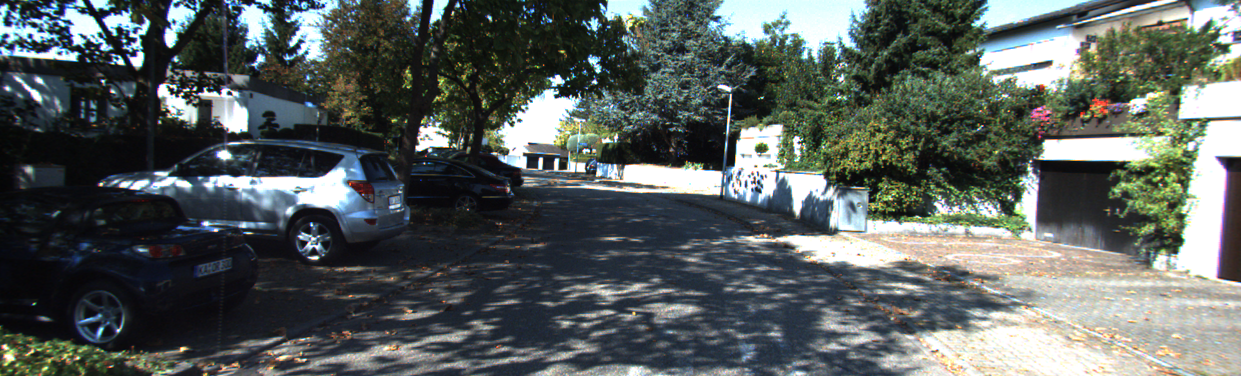
\includegraphics[width=0.7\linewidth]{base_img.png}
		\caption{Базовое изображение (uu\_000093.png).}
		\label{fig:base_img}
	\end{figure}

	\begin{figure}[p]
		\centering
		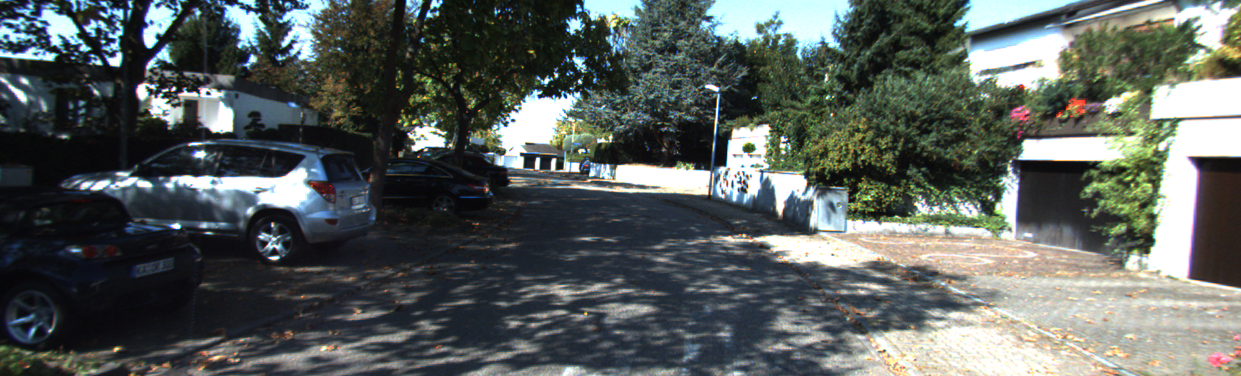
\includegraphics[width=0.7\linewidth]{pair_img.png}
		\caption{Парное изображение.}
		\label{fig:pair_img}
	\end{figure}

	\begin{figure}[p]
		\centering
		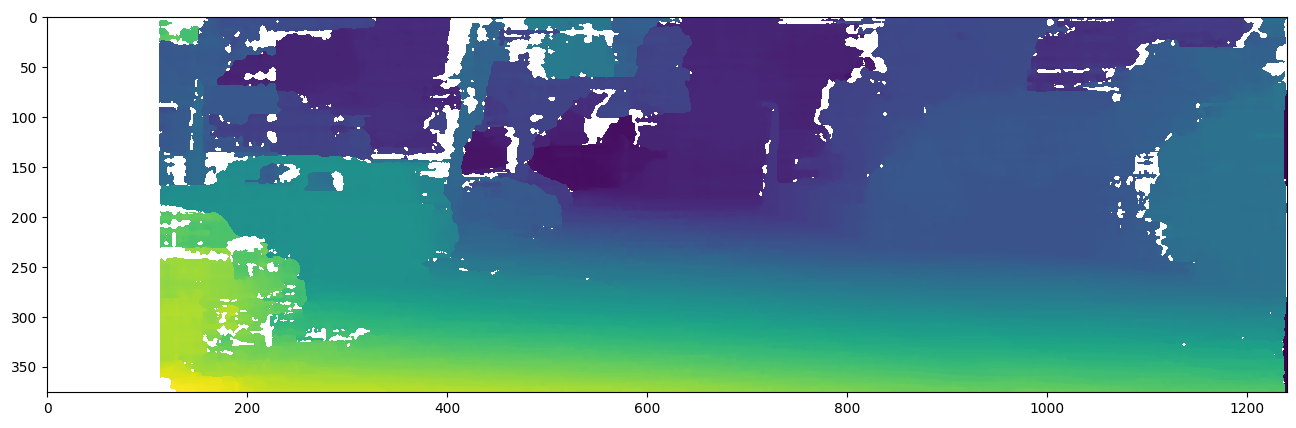
\includegraphics[width=0.75\linewidth]{disp_img.png}
		\caption{Карта диспаритета в псевдоцветах для базового изображения полученная с помощью алгоритма \texttt{cv::StereoSGBM}.}
		\label{fig:disp_img}
	\end{figure}

	\begin{figure}[p]
		\centering
		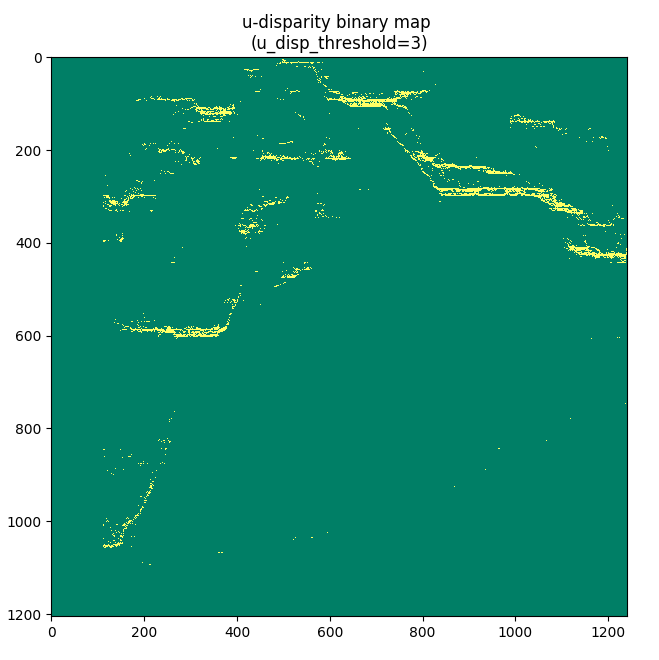
\includegraphics[width=0.7\linewidth]{u_disp.png}
		\caption{Бинаризованная с помощью порога карта u-диспаритета.}
		\label{fig:u_disp}
	\end{figure}

	\begin{figure}[p]
		\centering
		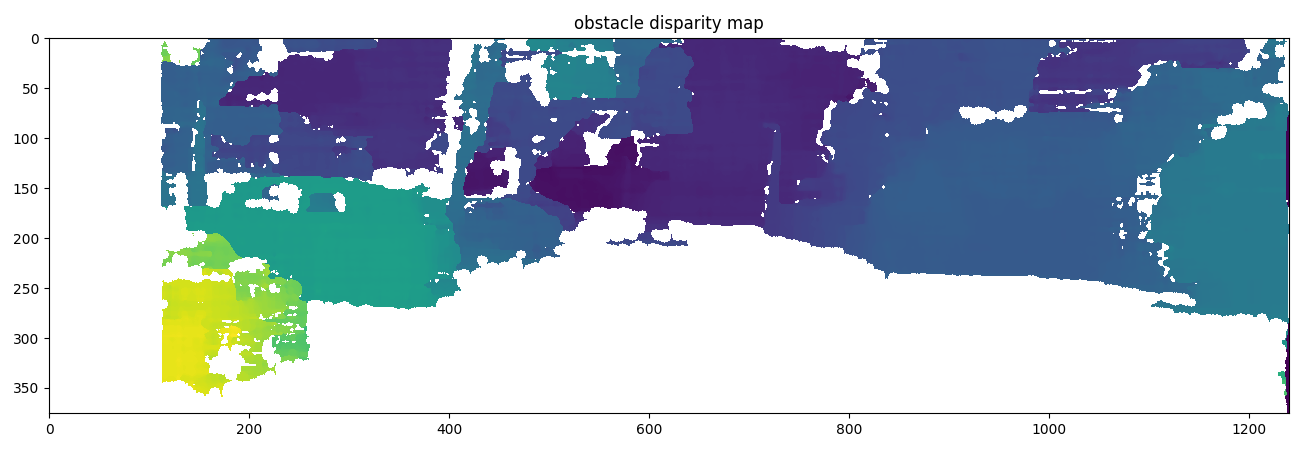
\includegraphics[width=0.7\linewidth]{obst_disp.png}
		\caption{Карта диспаритета препятствий.}
		\label{fig:obst_disp}
	\end{figure}

	\begin{figure}[p]
		\centering
		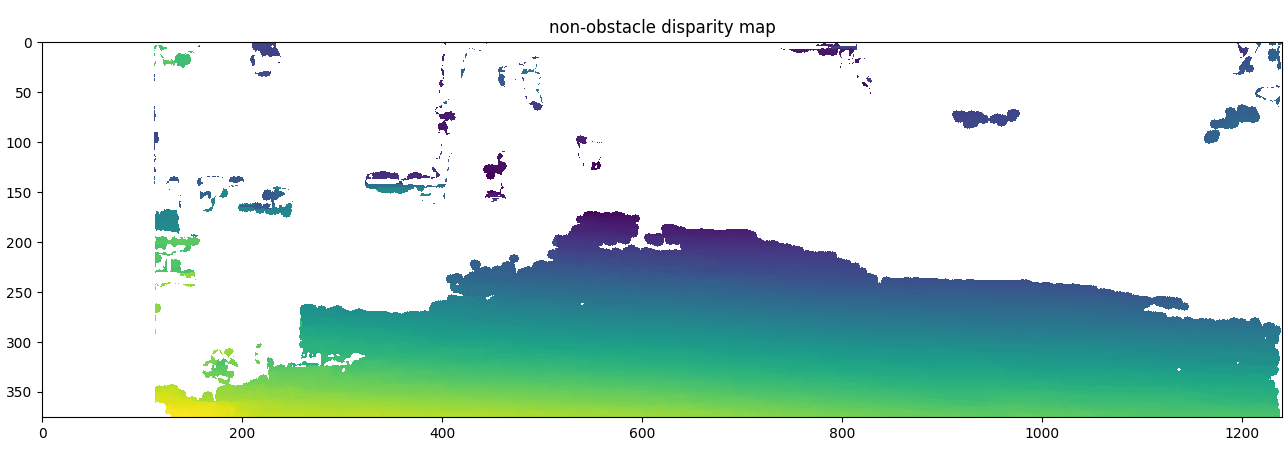
\includegraphics[width=0.7\linewidth]{non_obst_disp.png}
		\caption{Карта диспаритета не-препятствий.}
		\label{fig:non_obst_disp}
	\end{figure}

	\begin{figure}[p]
		\centering
		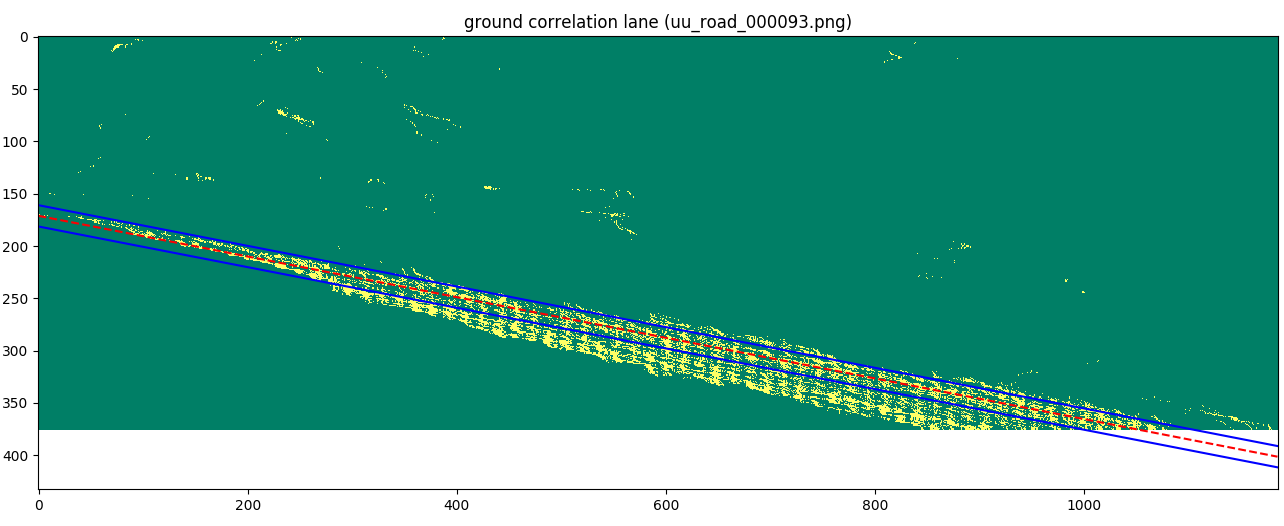
\includegraphics[width=0.7\linewidth]{gr_corelation.png}
		\caption{Нахождение линии корреляции земли на карте v-диспаритета (\(\texttt{line\_width=20}\)).}
		\label{fig:gr_corelation}
	\end{figure}

	\begin{figure}[p]
		\centering
		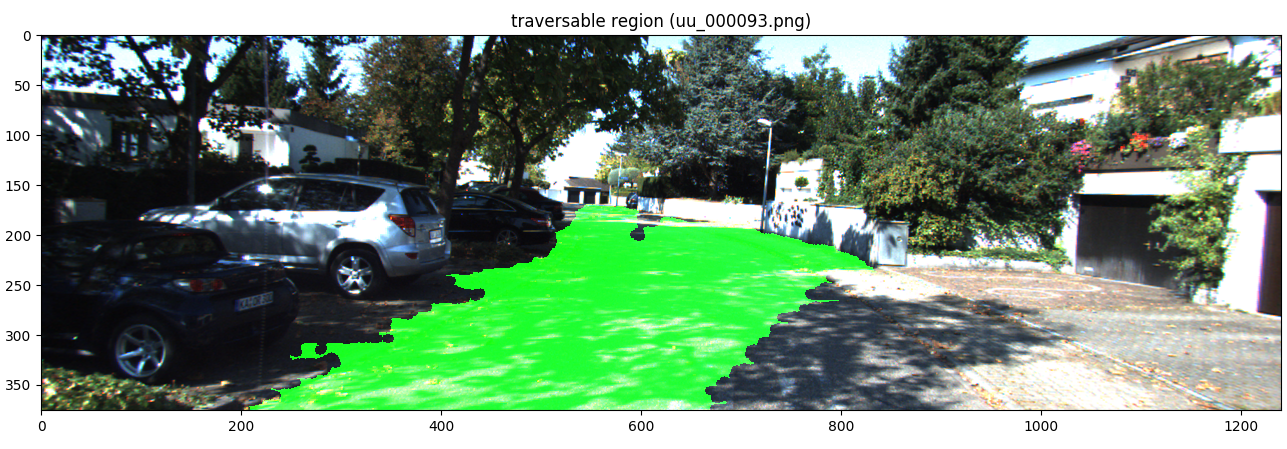
\includegraphics[width=0.7\linewidth]{img_with_tr_reg.png}
		\caption{Найденный регион для движения с использованием алгоритма (\(\texttt{line\_width=20}\)).}
		\label{fig:img_with_tr_reg}
	\end{figure}

	\begin{figure}[p]
		\centering
		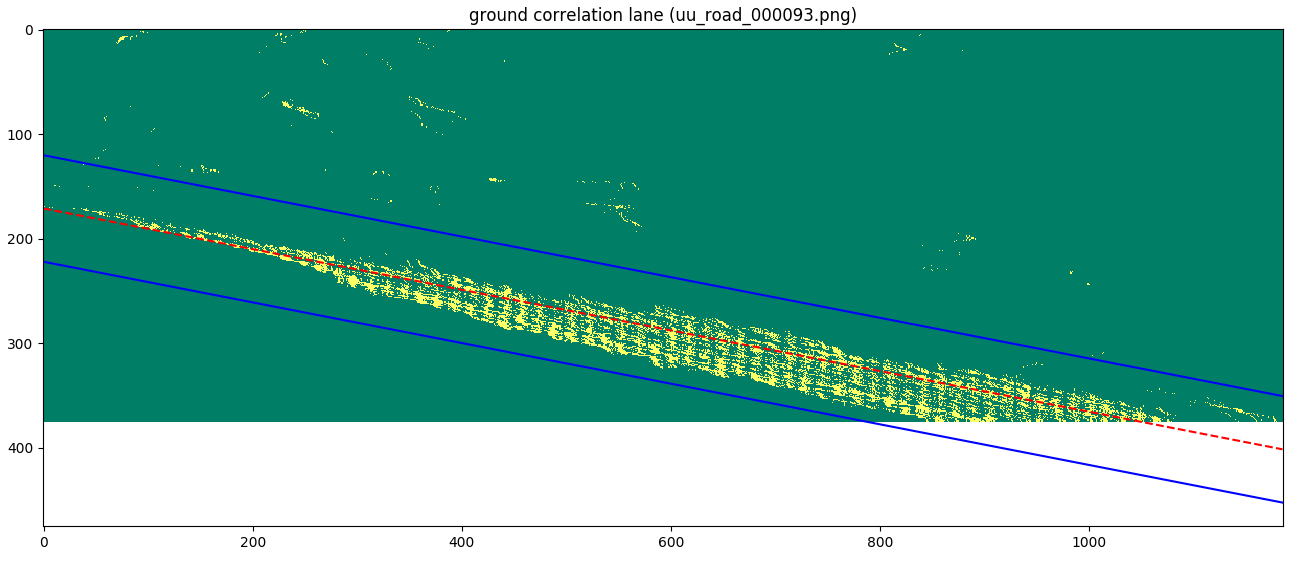
\includegraphics[width=0.7\linewidth]{gr_corelation_100.png}
		\caption{Нахождение линии корреляции земли на карте v-диспаритета (\(\texttt{line\_width=100}\)).}
		\label{fig:gr_corelation_100}
	\end{figure}

	\begin{figure}[p]
		\centering
		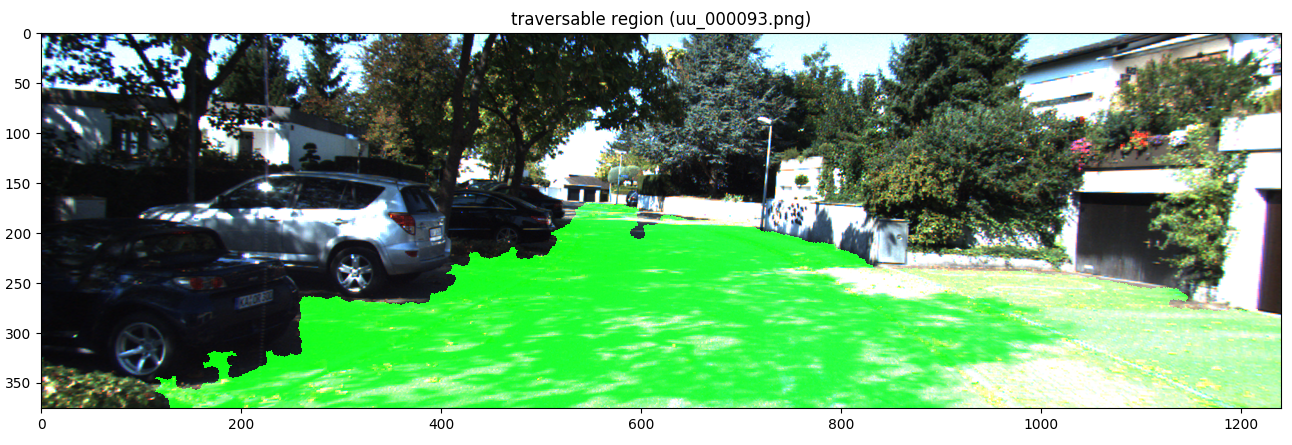
\includegraphics[width=0.7\linewidth]{img_with_tr_reg_100.png}
		\caption{Найденный регион для движения с использованием алгоритма (\(\texttt{line\_width=100}\)).}
		\label{fig:img_with_tr_reg_100}
	\end{figure}

	\begin{table}[p]
		\centering
		\caption{Характеристики работы алгоритма для карт диспаратности, полученных различными методами.}
		\label{tb:algs}
		\begin{tabular}{|c|c|c|c|c|c|c|}
			\hline
			\multicolumn{7}{|c|}{UM}  \\
			\hline
			\(\text{method}\) & \(\texttt{line\_width}\) & \(F_{max}(\%)\) & \(AvgPrec(\%)\) & \(Prec.(\%)\) & \(Recall(\%)\) & \(Acc.(\%)\) \\
			\hline
			StereoSGBM & 20 & \textbf{64.57} & \textbf{48.63} & \textbf{50.34} & 90.03 & \textbf{68.88} \\
			\hline
			ESGM & 20 & 63.63 & 46.33 & 47.82 & \textbf{95.07} & 65.76 \\
			\hline
			ELAS & 20 & 63.56 & 47.06 & 48.62 & 91.76 & 66.86 \\
			\hline
			\hline
			\multicolumn{7}{|c|}{UMM}  \\
			\hline
			\(\text{method}\) & \(\texttt{line\_width}\) & \(F_{max}(\%)\) & \(AvgPrec(\%)\) & \(Prec.(\%)\) & \(Recall(\%)\) & \(Acc.(\%)\) \\
			\hline
			StereoSGBM & 20 & 78.25 & \textbf{67.08} & \textbf{68.57} & 91.11 & \textbf{73.58} \\
			\hline
			ESGM & 20 & \textbf{78.82} & 65.84 & 67.21 & \textbf{95.29} & 73.29 \\
			\hline
			ELAS & 20 & 78.45 & 66.38 & 67.81 & 93.06 & 73.33 \\
			\hline
			\hline
			\multicolumn{7}{|c|}{UU}  \\
			\hline
			\(\text{method}\) & \(\texttt{line\_width}\) & \(F_{max}(\%)\) & \(AvgPrec(\%)\) & \(Prec.(\%)\) & \(Recall(\%)\) & \(Acc.(\%)\) \\
			\hline
			StereoSGBM  & 20 & 71.09 & 53.53 & 59.59 & 88.07 & 81.20 \\
			\hline
			ESGM & 20 & 71.96 & 55.57 & 58.50 & \textbf{93.47} & 80.89 \\
			\hline
			ELAS & 20 & \textbf{72.21} & \textbf{56.71} & \textbf{59.76} & 91.22 & \textbf{81.58} \\
			\hline
		\end{tabular}
	\end{table}

	\begin{table}[p]
		\centering
		\caption{Характеристики работы алгоритма для различных значений \(\texttt{line\_width}\).}
		\label{tb:l_width}
		\begin{tabular}{|c|c|c|c|c|c|c|}
			\hline
			%					\multicolumn{7}{|c|}{UM}  \\
			%					\hline
			\(\texttt{<cat>}\) & \(\texttt{line\_width}\) & \(F_{max} (\%)\) & \(AvgPrec (\%)\) & \(Prec. (\%)\) & \(Recall (\%)\) & \(Acc. (\%)\) \\
			\hline
			\hline
			\hline
			UM & 1 & 62.85 & \textbf57.65 & \textbf{79.45} & 52.00 & 80.64 \\
			\hline
			UM & 5 & \textbf{72.61} & \textbf{59.97} & 66.30 & 80.26 & \textbf{80.93} \\
			\hline
			UM & 10 & 69.40 & 52.83 & 57.57 & 87.33 & 75.74 \\
			\hline
			UM & 15 & 66.59 & 49.14 & 53.06 & 89.39 & 71.75 \\
			\hline
			UM & 20 & 64.57 & 48.63 & 50.34 & 90.03 & 68.88 \\
			\hline
			UM & 30 & 62.39 & 46.16 & 47.63 & 90.42 & 65.67 \\
			\hline
			UM & 40 & 61.35 & 45.05 & 46.41 & 90.50 & 64.08 \\
			\hline
			UM & 50 & 60.83 & 44.51 & 45.81 & \textbf{90.51} & 63.29  \\
			\hline
			UM & 60 & 60.44 & 44.11 & 45.37 & 90.51 & 62.68 \\
			\hline
			UM & 70 & 60.17 & 43.83 & 45.07 & 90.51 & 62.26 \\
			\hline
			UM & 80 & 59.99 & 43.65 & 44.86 & 90.51 & 61.97 \\
			\hline
			UM & 90 & 59.86 & 43.51 & 44.71 & 90.51 & 61.76 \\
			\hline
			UM & 100 & 59.79 & 43.44 & 44.64 & 90.51 & 61.65 \\
			\hline
			\hline
			\hline
			UMM & 1 & 68.57 & 68.20 & 52.17 & \textbf{100.00} & 52.17 \\
			\hline
			UMM & 5 & 77.47 & \textbf{71.67} & \textbf{78.98} & 76.01 & \textbf{76.93} \\
			\hline
			UMM & 10 & 78.93 & 69.75 & 73.66 & 85.01 & 76.32 \\
			\hline
			UMM & 15 & \textbf{78.94} & 67.35 & 70.72 & 89.32 & 75.14 \\
			\hline
			UMM & 20 & 78.25 & 67.08 & 68.57 & 91.11 & 73.58 \\
			\hline
			UMM & 30 & 77.18 & 64.86 & 66.13 & 92.66 & 71.41 \\
			\hline
			UMM & 40 & 76.50 & 63.78 & 64.94 & 93.08 & 70.17 \\
			\hline
			UMM & 50 & 76.04 & 63.12 & 64.22 & 93.20 & 69.36 \\
			\hline
			UMM & 60 & 75.89 & 62.91 & 63.99 & 93.23 & 69.10 \\
			\hline
			UMM & 70 & 75.78 & 62.77 & 63.83 & 93.24 & 68.91 \\
			\hline
			UMM & 80 & 75.72 & 62.69 & 63.74 & 93.25 & 68.80 \\
			\hline
			UMM & 90 & 75.67 & 62.62 & 63.67 & 93.25 & 68.72 \\
			\hline
			UMM & 100 & 75.64 & 62.59 & 63.63 & 93.25 & 68.67 \\
			\hline
			\hline
			\hline
			UU & 1 & 56.79 & 51.35 & \textbf{81.48} & 43.58 & 82.60 \\
			\hline
			UU & 5 & 71.35 & \textbf{59.09} & 71.41 & 71.29 & \textbf{84.98} \\
			\hline
			UU & 10 & \textbf{72.82} & 58.06 & 65.13 & 82.58 & 83.82 \\
			\hline
			UU & 15 & 71.79 & 55.11 & 61.52 & 86.18 & 82.23 \\
			\hline
			UU & 20 & 71.09 & 53.53 & 59.59 & 88.07 & 81.20  \\
			\hline
			UU & 30 & 69.99 & 51.80 & 57.48 & 89.46 & 79.87 \\
			\hline
			UU & 40 & 69.47 & 53.77 & 56.52 & 90.10 & 79.22 \\
			\hline
			UU & 50 & 69.15 & 53.29 & 55.99 & 90.38 & 78.83 \\
			\hline
			UU & 60 & 68.86 & 52.90 & 55.56 & 90.52 & 78.52 \\
			\hline
			UU & 70 & 68.71 & 52.70 & 55.34 & 90.59 & 78.35 \\
			\hline
			UU & 80 & 68.61 & 52.57 & 55.20 & 90.64 & 78.24 \\
			\hline
			UU & 90 & 68.56 & 52.49 & 55.12 & \textbf{90.67} & 78.17 \\
			\hline
			UU & 100 & 68.52 & 52.44 & 55.06 & 90.67 & 78.14 \\
			\hline
		\end{tabular}
	\end{table}


\newpage
\section*{Приложение. Исходный код программ}
\addcontentsline{toc}{section}{Приложение. Исходный код программ}
\label{app:}

	Исходный код скриптов на Python 3.6 доступен по адресу: \href{https://github.com/abramenko/traversable-region-detection}{https://github.com/abramenko/traversable-region-detection}

	Структура расположения файлов и папок представленна на Рис.~\ref{fig:repo_dir_struct}.

	\begin{figure}[h]
		\centering
		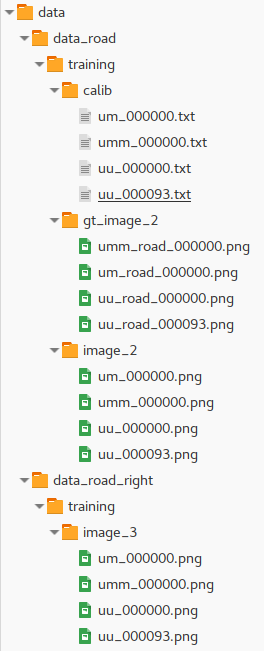
\includegraphics[width=0.3\linewidth]{repo_dir_struct_1.png}
		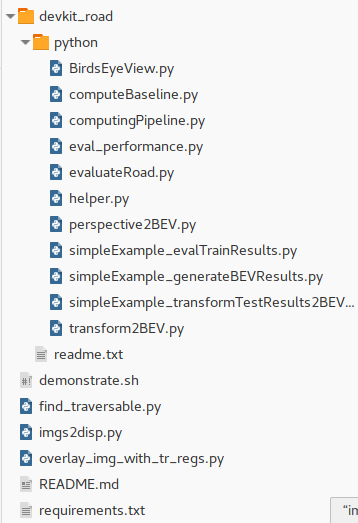
\includegraphics[width=0.4\linewidth]{repo_dir_struct_2.png}
		\caption{Структура расположения файлов и папок.}
		\label{fig:repo_dir_struct}
	\end{figure}

\end{document}


%---------------------------------------------------------------------
% Интервалы
%---------------------------------------------------------------------
%\renewcommand{\baselinestretch}{1.5}

% в преамбуле
%\usepackage{setspace}
%\onehalfspacing % полуторный интервал для всего текста
% или \singlespacing % одиночный интервал для всего текста
% или \doublespacing % двойной интервал для всего текста
% или \setstretch{множитель} % произвольный интервал

%% в тексте
%\begin{onehalfspace}
%фрагмент текста с полуторным межстрочным интервалом
%\end{onehalfspace}
%\begin{doublespace}
%фрагмент текста с двойным межстрочным интервалом
%\end{doublespace}

%---------------------------------------------------------------------


%--------------------------------------
%Нумерация
%--------------------------------------
%\pagestyle{empty} % нумерация выкл.
%\pagestyle{plain} % нумерация вкл.
%\thispagestyle{empty}% нумерация выкл.на странице

%--------------------------------------
%Если вдруг не работает нумирация:
%--------------------------------------
%\usepackage{fancyhdr}
%\pagestyle{fancy}
%\fancyhf{} % clear all header and footer fields
%\fancyhead[C]{\thepage}
%\renewcommand{\headrulewidth}{0pt}
%\renewcommand{\footrulewidth}{0pt}
% redefinition of the plain style:
%\fancypagestyle{plain}{%
%\fancyhf{} % clear all header and footer fields
%\fancyhead[C]{\thepage}
%\renewcommand{\headrulewidth}{0pt}
%\renewcommand{\footrulewidth}{0pt}}

%--------------------------------------
%Специальные символы
%--------------------------------------
% \ { } $ & # ^ _ % ~ "
% Команда \\ принудительно завершвет строку, но не завершает абзац
% Команда \noindent, вставленная перед непосредственно перед абзацем отменяет отступ
% Команда \par отделяет один абзац от другого
% \bigskip, \medskip e \smallskip -вставляют вертикальный интервал между обзацами
% "< -левая ёлочка
% "> -левая ёлочка
% "' -открывающая "лапка"
% "` -закрывающая "лапка"
% \' -ударение. Например больш\'ой
% \S -знак параграфа
% \No -знак номера
% ~   -неразрываемый пробел
% -
% --
% --- три вида тире

%--------------------------------------
%Генерация оглавления
%--------------------------------------
%\tableofcontents

%--------------------------------------
% Команды рубрикации
%--------------------------------------
%\chapter{title}
%\section{title}
%\subsection{title}
%\subsubsection{title}
%\paragraph{title}
%\subparagraph{title}
%\section*{От автора} %команды со звездочкой не влияют на нумерацию разделов и оглавление
%\addcontentsline{toc}{section}{От автора} %Принудительное добавление в оглавление

%--------------------------------------
%Управление формой шрифта(Декларирующие команды)
%--------------------------------------
%\sffamily %гарнитура без засечек (Sans Serif)
%\ttfamily %моноширинная гарнитура (Typewriter)
%\rmfamily %обычная гарнитура (Roman)
%\bfseries %включение ожирнения (bold face)
%\mdseries %отмена ожирнения (medium density)
%\itshape  %курсив (italics)
%\slshape  %наклонный шрифт(slanted)
%\scshape  %капитель (small caps)
%\upshape  %обычное начертание (upright)
%\normalfont % основной шрифт документа
%\emph{} %выделение(emphasis)

%--------------------------------------
%Управление формой шрифта(Команды с параметром)
%--------------------------------------
%\textsf{} \texttt{} \textrm{} \textbf{} \textmd{} \textit{} \textsl{} \textsc{} \textup{} \textnormal{}

%--------------------------------------
%Управление формой шрифта(Команды в форме окружения)
%--------------------------------------
%\begin{bfseries}
%		Текст к которому применить
%\end{bfseries}

%--------------------------------------
%Управление размером шрифта
%--------------------------------------
%\tiny \scriptsize \footnotesize \small \normalsize \large \Large \LARGE \huge \Huge

%--------------------------------------
%Перекрестные ссылки
%--------------------------------------
%\label{key} % метка
%\ref{{main:theorem:prove} % возвращает номер параграфа, в котором стоит метка
%\pageref{{main:theorem} % возвращает номер страницы, на которой стоит метка

%--------------------------------------
%Список литературы и ссылки на него
%--------------------------------------
%\begin{thebibliography}{00}
%  \bibitem[<номер(необязательный параметр)>]{<метка>}
%  \bibitem{autor} Авторы книги. \emph{Название книги.} Издательство,город , год издания.
%  \bibitem{autor} Авторы статьи. \emph{Название статьи.}//\emph{Название сборника}стр.~111--123. Издательство,город, год издания.
%\end{thebibliography}
%\cite[<дополнительный текст. Например: стр.~27>]{<метка источника, на который ссылаемся>} - вставляет в текст ссылку

%--------------------------------------
%Оформление приложений
%--------------------------------------
%\appendix
%\chapter{Заголовок приложения}

%--------------------------------------
% НЕ нумерованные перечисления
%--------------------------------------
% \begin{itemize}
% 	\item Один
% 	\item Два
% \end{itemize}

%--------------------------------------
% Нумерованные перечисления
%--------------------------------------
%\begin{enumerate}
%	\item Один
%	\item Два
%\end{enumerate}

%--------------------------------------
%Описание плавающих объектов(картинки,таблицы)
%--------------------------------------
%\begin{table}[дополнительные параметры]
% ... Описание таблицы ...
%\caption{Название таблицы}
%\label{метка этой таблицы}
%\end{table}
%----------
%\begin{figure}[дополнительные параметры]
% ... Описание рисунка ...
%\caption{название рисунка}
%\label{метка этого рисунка}
%\end{figure}
%----------
%Сослаться можно так:
%см.~табл.\,\ref{метка этой таблицы} на стр.\,\pageref{метка этой таблицы}


%--------------------------------------
%Управление размещением объектов
%--------------------------------------
%\begin{figure}[hp] - по возможности поставить в месте появления или же на отдельной странице
% t - размещение в верхней части страницы(top)
% b - в нижней части(bottom)
% p - на отдельной странице(page)
% h - сразу же после появления в тексте(here)
% ---------
% Пожелание можно превратить в требование добавив восклецательный знак:
% \begin{figure}[h!]

%--------------------------------------
%Пример создания таблицы:
%--------------------------------------
%\begin{table}[t]
%\begin{tabular}{|r|c|p{5cm}|
%p{0.25\textwidth}|p{40pt}|l|}
%\hline \No & Тип & Автор & Заглавие & Год & Тираж \\ \hline
%1 & книга & Артур Конан Дойл & Собака Баскервилей & 1975 & 10\,000 \\ \hline
%2 & книга & Жуль Верн & Пять недель на воздушном шаре & 1981 & 7000 \\ \hline
%3 & журнал & \multicolumn{2}{c|}{Вокруг света (\No 5)}& 1995 & 5000 \\ \hline
%\end{tabular}
%\caption{пример таблицы}
%\label{sample_table}
%\end{table}
%-------
%\hline -разделяет строки таблиы горизонтальной чертой
%\сline{2-4} -проведет горизонтальную черту через столбцы со второго по четвертый

%--------------------------------------
%Пример импорта рисунка
%--------------------------------------
%\begin{figure}[t]
%\centering
%\includegraphics[width=0.9\textwidth]{2014}
%\caption{2014 example}
%\label{truck_figure}
%\end{figure}

%--------------------------------------
% Оформляем листинги программ
%--------------------------------------
%\begin{verbatim}
%    int main()
%    {
%        return 0;
%    }
%\ end{verbatim}
%Для однострочных вставок можно использовать \verb: некоторый текст :
% Или \texttt{некоторый текст}
% Так же есть \verb* и \begin{verbatim*}
%---------
%Пакет verbatim позволяет включать текст из внешнего файла
%\usepackage{verbatim}
%\verbatiminput{<имя файла>}
%---------
%Пакет spverbatim делает breakline
%\begin{spverbatim}
%Long text
%\ end{spverbatim}
%Пакет moreverb позволяет нумировать всавляемые строки в листинге
%\usepackage{moreverb}
%\begin{listing}[<шаг>]{<старт>}
%  int main()
%  {
%      return 0;
%  }
%\ end{listing}
%Вставка из файла
%\usepackage{moreverb}
%\listinginput[<шаг>]{<старт>}{<имя файла>}
%Так же существуют команды \listinginput* и \begin{listing*}
%\begin{lstlisting}
%Put your code here.
%\ end{lstlisting}
%--------
%Еще один пакет для листинга
%\usepackage{listings}
%\lstinputlisting[language=C++, frame=L, breaklines=true]{main.cpp}
%ИЛИ
%\usepackage{listings}
%\lstinputlisting[language=C++, frame=single]{main.cpp}
%ИЛИ
%\usepackage{listings}
%\usepackage{color}
%\lstdefinestyle{customc}{belowcaptionskip=1\baselineskip, breaklines=true, frame=L, xleftmargin=\parindent, language=C++, showstringspaces=false, basicstyle=\footnotesize\ttfamily,keywordstyle=\bfseries\color{blue}, commentstyle=\itshape\color[gray]{0.5}, identifierstyle=\color{black}, stringstyle=\color[RGB]{125,25,0}}
%\lstinputlisting[style=customc]{main.cpp}
%ИЛИ
%\usepackage{listings}
%%\lstset{
%language=C,                 % выбор языка для подсветки (здесь это С)
%basicstyle=\small\sffamily, % размер и начертание шрифта для подсветки кода
%numbers=left,               % где поставить нумерацию строк (слева\справа)
%numberstyle=\tiny,           % размер шрифта для номеров строк
%stepnumber=1,                   % размер шага между двумя номерами строк
%numbersep=5pt,                % как далеко отстоят номера строк от подсвечиваемого кода
%backgroundcolor=\color{white}, % цвет фона подсветки - используем \usepackage{color}
%showspaces=false,            % показывать или нет пробелы специальными отступами
%showstringspaces=false,      % показывать или нет пробелы в строках
%showtabs=false,             % показывать или нет табуляцию в строках
%frame=single,              % рисовать рамку вокруг кода
%tabsize=2,                 % размер табуляции по умолчанию равен 2 пробелам
%captionpos=t,              % позиция заголовка вверху [t] или внизу [b]
%breaklines=true,           % автоматически переносить строки (да\нет)
%breakatwhitespace=false, % переносить строки только если есть пробел
%escapeinside={\%*}{*)}   % если нужно добавить комментарии в коде
%}
%\begin{lstlisting}
%    текст тут
%\ end{lstlisting}

%--------------------------------------
%Добавим цвет
%--------------------------------------
%\usepackage{color}
%{\color[RGB]{255,0,0} This text will appear red-colored}
%\pagecolor{green}
%\colorbox[gray]{0.5}{text}
%\colorbox[rgb]{0,1,0}{text}

%--------------------------------------
%Гиперссылки
%--------------------------------------
%\usepackage{hyperref} или \usepackage[pdftex]{hyperref}
%\href{http://www.wikibooks.org}{Wikibooks home}
%\url{http://www.wikibooks.org}
%\hyperlink{label}{link caption}
%\hypertarget{label}{target caption}

%--------------------------------------
%Сноски
%--------------------------------------
%\footnote{text}
%\footnote{Первая сноска}\label{my_footnote}
%\footnotemark{\ref{my_footnote}}

%--------------------------------------
%Текст и знаки на полях
%--------------------------------------
%\marginpar{<текст>}
%-----
%Значек "восклицательный знак"
%Описание
%\newcommand\attentionpicture{
%\begin{picture}(20,20)(0,0)
%\put(0,0){\line(1,0){20}}
%\put(0,0){\line(2,3){10}}
%\put(20,0){\line(-2,3){10}}
%\put(8.3,3){\bf !}
%\end{picture}
%}
%\newcommand\attention{
%\marginpar[\hfill\attentionpicture]
%{\attentionpicture}
%}
%Вызов
%\attention

%--------------------------------------
%Математичекий режим
%--------------------------------------
%--------------------------------------
%Вставка формулы
%--------------------------------------
%Непосредственно в текст
%\begin{math}
%\int_0^{2\pi}{\frac{\sin x}{x}dx}
%\end{math}
%Короткая команда:
%\( ... \) или $ ... $
%------
%На отдельной строке
%\begin{displaymath}
%\int_0^{2\pi}{\frac{\sin x}{x}dx}
%\end{displaymath}
%Короткая команда:
%\[ ... \] или $$ ... $$
%------
%На отдельной строке с нумерацией формулы
%\begin{equation}
%\int_0^{2\pi}{\frac{\sin x}{x}dx}
%\end{equation}
%------
%Для расстаноки пробелов, можно использовать команды:
% \  или \; или \: или \quad или \qquad
%Существуют отрицательные пробелы:
% \negthinspace, \!, \negmedspace и \negthickspace
%------
%--------------------------------------
%Пакет amsmath
%--------------------------------------
%\usepackage{amsmath}
%\[ V_\text{сближения} = V_\text{автомобиля} + V_\text{сближения} \]
%\( \frac{x+\frac{1}{y}}{\frac{z+1}{3}-15} \)
%\sqrt[3]{a+b}
%\[ \sqrt{ x_1 + \sqrt{ x_2 + \sqrt{ x_3 }}} \]
%--------------------------------------
%Символы больших операторов
%--------------------------------------
%\( 1\int 2\oint 3\sum 4\prod 5\coprod 6\bigcap 7\bigcup 8\bigsqcup 9\bigoplus 10\bigotimes 11\bigodot 12\biguplus 13\bigvee 14\bigwedge \)
%--------------------------------------
%Наиболее употребляемые математические символы
%--------------------------------------
%\( 15 \forall 16 \exists 17 \infty 18 \mapsto 19 \emptyset 20 \nabla 21 \in 22 \ni 23 \sim 24 \subset 25 \supset 26 \setminus 27 \subseteq 28 \supseteq 29 \equiv 30 \leq 31 \geq 32 \neq 33 \cdot 34 \approx 35 \cong 36 \ll 37 \gg 38 \mid 39 \vee 40 \wedge 41 \triangle 42 \perp 43 \parallel 44 \angle 45 \lfloor 46 \rfloor 47 \partial 48 \lceil 49 \rceil 50 \neg 51 \pm 52 \mp 53 \times 54 \cap 55 \cup 56 \div 57 \oplus 58 \ominus 59 \otimes 60 \oslash 61 \odot 62 \circ \)
%--------------------------------------
%Разные стрелочки
%--------------------------------------
%\( 63 \leftarrow 64 \rightarrow 65 \Leftarrow 66 \Rightarrow 67 \leftrightarrow 68 \Leftrightarrow 69 \longleftarrow 70 \longrightarrow 71 \Longleftarrow  72 \longleftrightarrow 73 \Longrightarrow 74 \Longleftrightarrow \)
%--------------------------------------
%Греческие буквы
%--------------------------------------
%\noindent\( 75\ \alpha\ 76\ \beta\ 77\ \gamma\ 78\ \delta\ 79\ \epsilon\ 80\ \varepsilon\ 81\ \zeta\ 82\ \eta\ 83\ \theta\ 84\ \vartheta\ 85\ \iota\\ 86\ \kappa\ 87\ \lambda\ 88\ \mu\ 89\ \nu\ 90\ \xi\ 91\ \pi\ 92\ \varpi\ 93\ \rho\ 94\ \varrho\ 95\ \sigma\ 96\ \varsigma\ 97\ \tau\\ 98\ \upsilon\ 99\ \phi\ 100\ \varphi\ 101\ \chi\ 102\ \psi\ 103\ \omega\ 104\ \Gamma\ 105\ \Delta\ 106\ \Theta\ 107\ \Lambda\\ 108\ \Xi\ 109\ \Pi\ 110\ \Sigma\ 111\ \Upsilon\ 112\ \Phi\ 113\ \Psi\ 114\ \Omega \)
%--------------------------------------
%Расстановка приделов больших операторов
%--------------------------------------
%\[\sum_{i=0}^{n} q_i\]
%Располагаем приделы над знаком оператора или рядом:
%\[\int\limits_a^b f(x)\,dx\]
%\[\sum\nolimits_{i=0}^{n}q_i\]
%--------------------------------------
%Кратные интегралы
%--------------------------------------
%\iint  \iiint \iiiint \idotsint
%--------------------------------------
%Отрицание логических символов
%--------------------------------------
%\(x \not\in T\)
%\(x \not< y\)
%--------------------------------------
%Пакет amsfonts
%--------------------------------------
%--------------------------------------
%Математические шрифты
%--------------------------------------
%\usepackage{amsfonts}
%\begin{document}
%\(
%%Каллиграфический
%\mathcal{ABCDEFGHIJKLMNOPQRSTUVWXUZ}\\
%%Готический
%\mathfrak{ABCDEFGHIJKLMNOPQRSTUVWXUZ}\\
%\mathfrak{abcdefghijklmnopqrstuvwxuz}\\
%%Ажурный
%\mathbb{ABCDEFGHIJKLMNOPQRSTUVWXUZ}\\
%\)
%\end{document}
%--------------------------------------
%Акценты в формулах
%--------------------------------------
%\(1\ \hat x\ 2\ \check x\ 3\ \acute x\ 4\ \grave x\ 5\ \dot x\ 6\ \ddot x\ 7\ \dddot x\ 8\ \ddddot x\ 9\ \bar x\ 10\ \vec x\ 11\ \breve x\ 12\ \tilde x\ 13\ \mathring x\ \)
%--------------------------------------
%Многоточие
%--------------------------------------
%\ldots % -точки вдоль низа строки
%\cdots % -точки вдоль середины строки
%\vdots % - вертикальное многоточие
%\ddots % -диагональное многоточие
%--------------------------------------
%Математические скобки
%--------------------------------------
% 1\ (x + y) \\
% 2\ \langle x+y \rangle \\
% 3\ [x + y] \\
% 4\ \lfloor x+y \rfloor \\
% 5\ \{x+y\} \\
% 6\ \lceil x+y \rceil
%--------------------------------------
%Символы-ограничители
%--------------------------------------
% /
% \backslash
% |
% \|
% \uparrow
% \Uparrow
% \downarrow
% \Downarrow
% \updownarrow
% \Updownarrow
%--------------------------------------
%Управление размером скобок
%--------------------------------------
%\bigl(\text{какой-то текст} \bigm | \text{ещё текст} \bigr)
%\big
%\Big
%\bigg
%\Bigg
%\Bigl..\Bigm..\Bigr
%\biggl..\\biggm..\biggr
%\Biggl..\Biggm..\Biggr
%\left( ... \right) %-автоматическое управление размером
%\left.  %- нулевой ограничитель
%\right. %- нулевой ограничитель
%\left\{...\right.
%--------------------------------------
%Дополнительные математические символы
%--------------------------------------
%Пример некоторых символов из пакета amssymb
%\usepackage{amssymb}
%1 \leqslant 2 \geqslant 3 \lll 4 \ggg 5 \lessdot 6 \gtrdot 7 \fallingdotseq 8 \risingdotseq 9 \doteqdot 10 \vDash 11	 \circlearrowleft 12 \curvearrowleft
%--------------------------------------
%Знаки "больше или равно", "меньше или равно"
%--------------------------------------
%\leq и \geq
%--------------------------------------
%Ручная установка стилей формул
%--------------------------------------
%\displaystyle
%\textstyle
%\scriptstyle
%\scriptscriptstyle
%Пример:
%\[
%1+\frac{1}{\displaystyle 1+
%\frac{1}{\displaystyle 1+
%\frac{1}{\displaystyle 1+
%\frac{1}{x}}}} \]
%--------------------------------------
% Матрицы
%--------------------------------------
% Оганичивающие скобки в явном виде
% \[ \left( \begin{matrix}
% 1 & 2 & 3 \\ x & y & z \\ a & b & c \\
% \end{matrix} \right) \]
%--------
% Матрица вместе с ограничителями
% pmatrix
% bmatrix
% vmatrix
% Vmatrix
%Пример:
%\(\begin{pmatrix} a_1^1 & a_1^2 \\ a_2^1 & a_2^2 \end{pmatrix}\)
%--------
% Матрица - строчная форма
%\(\left( \begin{smallmatrix} a & b \\ c & d \end{smallmatrix} \right)\)
%--------------------------------------
% Максимальная ширина матриц (10 столбцов)
%--------------------------------------
%\setcounter{MaxMatrixCols}{20} % - увеличение максимальной ширины. Чем больше значение, тем больше времени тратится на верстку документа
%--------------------------------------
% Группа формул с выравниванием
%--------------------------------------
% Точка выравнивания задается символом &
% \[ \begin{aligned}
% \sin x\pm\sin y& = 2\sin\frac{x\pm y}{2}\cos\frac{x\mp y}{2}\\
% \sin x\sin y & = \frac{1}{2}(\cos(x-y)-\cos(x+y))\\
% \end{aligned} \]
%--------------------------------------
% Система уравнений и неравенств
%--------------------------------------
%\begin{align}
%M_{00} &=\left( a+b\right) \frac{\pi R^{2} }{2} +\left( a-b\right) \left( p\sqrt{R^{2} -t^{2} } +R^{2} \arcsin \frac{t}{R} \right)  ,\\
%M_{10} &=-\frac{a-b}{3} \sqrt{R^{2} -t^{2} } \left( 2R^{2} -pt-p^{2} \right)  ,\\
%M_{20} &=\frac{a+b}{2} \cdot \frac{\pi R^{4} }{4} -\left( a-b\right) \left[ \frac{1}{6} \sqrt{R^{2} -t^{2} } \left( \frac{3}{2} R^{2} t-pt^{2} -tp^{2} -p^{3} \right) -\frac{R^{4} }{4} \arcsin \frac{t}{R} \right]  ,\\
%M_{02} &=\frac{a+b}{2} \cdot \frac{\pi R^{4} }{4} -\left( a-b\right) \left[ \frac{1}{6} \sqrt{R^{2} -t^{2} } \left( pt^{2} -R^{2} p-\frac{3}{2} R^{2} t\right) -\frac{R^{4} }{4} \arcsin \frac{t}{R} \right] \nonumber .
%\end{align}

% \[ \left\{\begin{aligned}
% & x+y=5 \\ & x-2y=2
% \end{aligned}\right. \]
%ИЛИ
% \[ \left|\begin{aligned}
% & x < 5 \\ & x > 15
% \end{aligned}\right. \]
%--------------------------------------
% Перечисление случаев
%--------------------------------------
% \[ |x| = \begin{cases}
% x, & x \ge 0, \\
% -x, & x < 0
% \end{cases} \]
%--------------------------------------
% Подписанные знаки отношений
%--------------------------------------
% \(
% \ln x\stackrel{\text{Df}}{=}y,\, e^y=x
% X \stackrel{\alpha} {\longrightarrow} Y
% \)
% \xleftarrow и \xrightarrow %- стрелки, которые меняют размер, в зависимости от подписи.
%\[ f(x,y) \xrightarrow[D\rightarrow D_0] {(x,y)\in D} 0 \]
%--------------------------------------
% Многострочные индексы
%--------------------------------------
% \[\lim_{\substack{
% x\rightarrow 0 \\
% y\rightarrow 0 \\
% z\rightarrow 0}} F(x,y,z)
% \])
%----------
% Выравнивание по левому краю
% \[
% \idotsint\limits_{
% \begin{subarray}{l}
% x \in V \\ \tau(x)>0
% \end{subarray}} \varphi\,ds
% \]
%--------------------------------------
% Как верстать титульную страницу (latex3days.pdf стр.81)
%--------------------------------------
% Центрирование текста
%\centerline{Некий текст}
%\begin{center}
%Еще текст
%\end{center}
%--------------------------------------
% Пропуск места по вертали и горизонтали
%--------------------------------------
%Промежуток фиксированного размера
%\vskip2cm
%\vskip15mm
%\vskip1.5pt
%------
%Равномерное распределение вертикального пространства
%\vfill
%------
%Фиксированный горизонтальный отступ
%\hspace{<длинна>}
%\hspace*{<длинна>}
%------
%Равномерный горизонтальный отступ
%\hfill
%--------------------------------------
% Горизонтальное отчеркивание
%--------------------------------------
%\rule[<высота>]{<длина>}{<толщина>}
%\hrulefill %Динамическое
%--------------------------------------
% Выравнивание по правому краю
%--------------------------------------
%\rightline{<строка>}
%------
%\begin{flushright}
%Пошла вода\\
%в хату.
%\end{flushright}
%--------------------------------------
% Министраницы
%--------------------------------------
%\null\hfill
%\begin{minipage}{0.3\textwidth}
%Это текст будет прижат к равому краю страницы
%\end{minipage}\\
%--------------
%\null\hfill
%\begin{minipage}{0.3\textwidth}
%\fbox{Текст, который в рамке и прижат к правому краю страницы}
%\end{minipage}\\
%--------------------------------------
% Как закончить титульную страницу
%--------------------------------------
%\clearpage
%\thispagestyle{empty} % ненумеруем эту страницу
%------
%\begin{titlepage}
%содержимое...
%\end{titlepage}
%\setcounter{page}{2} %Нумерация со второй страницы